\documentclass[a4paper,pra,twocolumn,10pt,aps,longbibliography,nobalancelastpage]{revtex4-1}


\usepackage{graphicx}
\usepackage{caption}
\usepackage{subcaption}
\usepackage{amsmath}
\usepackage{minted}
\usepackage{listings}
\usepackage{units}
\usepackage{balance}
\begin{document}
\title{Real-Time Digital Signal Processing Final Project}
\author{Ahmad Moniri, CID: 00842685, and Pranav Malhotra, CID: 00823617}
\date{21st March 2016}

\begin{abstract}
Real-time speech enhancement is vital in almost all aspects of life. Estimating the spectrum of noise and subtracting it from the spectrum of the corrupted signal, a process known as spectral subtraction, is widely used to improve the quality of speech signals. There are multiple trade-offs that have to be carefully weighed before a sound algorithm that is flexible enough to deal with any speech signal, yet effective at eliminating all types of noise, can be implemented.
\end{abstract}

\maketitle
\section{Theory}\label{sec:theory} 
For spectral subtraction to be properly implemented, the signal needs to be processed in the frequency domain. The signal is assumed to be corrupted by additive noise and thus its magnitude spectrum is a linear combination of the magnitude spectrum of the original signal and the magnitude spectrum of the noise. \textbf{Although the noise is assumed to be additive, the spectral subtraction methodology does not require the noise to be white. Neither is a priori knowledge of the probability density function (PDF) necessary.} Lastly, the spectral subtraction algorithm only improves the magnitude spectrum of the signal; the phase spectrum is left unaltered. A block diagram that outlines the speech enhancement process is presented in figure \ref{fig:spec_sub_overview}.

\begin{figure}[H]
    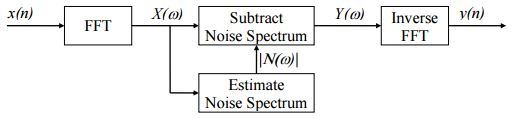
\includegraphics[width=\columnwidth]{spec_sub_overview}
    \caption{Overview of spectral subtraction process}
    \label{fig:spec_sub_overview}
\end{figure}

Noise estimation is done over a 10 second moving window. It is safe to assume that the speaker will pause at some point in the 10 second period. When the speaker is paused, the signal will only consist of the background noise that needs to be removed. The power of the signal will be minimum at this point. The noise is estimated by identifying the minimum  magnitude spectrum. A scaling factor, $\alpha$, is introduced to ensure that sufficient noise is removed. Different algorithms estimate the noise spectrum differently and thus the scaling factor will depend on the algorithm used; in almost all scenarios, the estimated value of the noise is significantly lesser than the actual noise and thus $\alpha$ is usually more than 1. $\alpha$ is more commonly in the range [5, 20].

The processing is performed in real time. For real-time processing to be possible, the signal has to be divided into small overlapping frames. To ensure that the overlapping of the frames does not introduce distortion, an overlap-add algorithm is used to form the output signal. In addition, a window is applied to smoothen the frame such that sharp changes in the time domain due to the finite length nature of the sequence are removed. For the Real-Time Digital Signal Processing Final Project, the square root of the Hanning window will be used to window the signal.

Next, it is important to note that the time available for processing is dependent on how often new data is read. The default frame length is 256. A quarter frame is read every 8ms and this sets the upper limit on the time available for processing. In addition, note that although a new set of data contains only 64 samples, the processing is performed with 256 samples; the oversampling rate is 4.\textbf{ The oversampling allows the Fourier Transform to be evaluated at 4 times the number of frequencies than if oversampling was not performed and thus improves the frequency resolution.} Moreover, the changes in the magnitude spectrum if oversampling is used are gradual as 75\% of the 256 time domain samples are identical to the samples in the previous frame. \textbf{Note that, although 75\% of the time domain samples, in adjacent frames, are identical, 75\% of the magnitude spectrum is not going to be identical.} It is more likely that none of the frequencies at which the Fourier Transform is evaluated have the same magnitude. However, the change in the Fourier Transform from frame to frame will be gradual, not sharp.


\section{Experimentation}
\subsection{Basic Algorithm}
The skeleton code provided performs the input and output buffering. The overlap-add algorithm required to compute the output has also been implemented. Only the frame processing algorithm needs implementing. As in laboratory 5, the memory required to hold data will be dynamically allocated. In addition header files including helper functions that provide support in dealing with complex numbers have been provided.

\subsubsection{FFT}
Listing \ref{lst:fft} presents how the input data is converted into a complex number. The complex number template requires both the real and the imaginary part of the number to be specified at initialisation. Since the signals that are processed in this course are all real, the imaginary part is set to zero. The function {\tt fft} is called and it operates on the vector {\tt X}. The FFT obtained will be a complex number since the input consists of both sine and cosine components. As discussed in section \ref{sec:theory}, the signal will be processed in the frequency domain. \textbf{The frequency domain is two dimensional and only 1 dimension, namely the magnitude spectrum will be manipulated.} To operate on the magnitude spectrum, the function {\tt cabs} is utilised.

\begin{listing}[H]
\begin{minted}[fontsize=\scriptsize]{C}
// Convert inframe into complex number
// X initialised to be a complex buffer
for (i=0; i<FFTLEN; i++){                           
    X[i] = cmplx(inframe[i], 0);
} 

// Take fft
fft(FFTLEN, X);

// Obtain absolute value of complex number
// cabs_X initialised to be a floating point bufeer
for (i=0; i<FFTLEN; i++){                           
    cabs_X[i] = cabs(X[k]);
} 
\end{minted}
\caption{FFT of {\tt inframe}} 
\label{lst:fft}
\end{listing}

\subsection{Estimation of Noise}\label{sec:noise_est}
As discussed, the noise will be estimated over a 10 second window. \textbf{Although the system has 10 seconds of memory, it is not feasible to store 10 seconds of data; only relevant data will be stored.} The aim of the noise estimation process is to identify the minimum magnitude of each frequency bin over the 10 second period. As a whole, this will be referred to as the minimum magnitude spectrum and it will indicate the spectral components that the noise contributes. 

In the Real-Time Digital Signal Processing coursework it is suggested that the 10 second window is split into 4 smaller 2.5 second windows. For each 2.5 seconds window, only the minimum magnitude spectrum is stored. Such an implementation will significantly reduce the amount of memory the program requires. The number of buffers determine how responsive the system is to noise that is non-stationary. With 4 buffers, an individual buffer will store the minimum magnitude spectrum over a 2.5 seconds. To allow the system to have a greater amount of flexibility, the number of buffers can be increased. For example, if 10 buffers were used, each buffer would hold the magnitude spectrum over a 1 second window. The increased flexibility does have some overhead in the form of increased memory requirements. In addition, buffer rotation, described below, will have to be performed more often; described in section \ref{sec:noise_filter} are the effects of performing buffer rotation on the quality of the signal. 

Since all processing is performed with 256 samples, the buffers that store the minimum magnitude spectrum will also be 256 in size. Next, since the processing is done on the magnitude spectrum, the buffers will be declared as floats. Dynamically allocated buffers are initialised to 0 however the buffers that hold the minimum magnitude spectrum are initialised to {\tt FLT\_MAX}; this is necessary to ensure that it does not take 10 seconds for the system to identify the noise and start the spectral subtraction process. 

If 4 buffers are used, they have to be rotated every 2.5 seconds; the buffer containing the oldest data will be reset to {\tt FLT\_MAX}. The buffers are updated by changing the address of the pointers {\tt M\_1}, {\tt M\_2}, {\tt M\_3} and {\tt M\_4}, rather than through manual reading and writing of data from one memory location to another. The C code that implements buffer rotation is presented in listing \ref{lst:buff_rot}

\begin{listing}[H]
\begin{minted}[fontsize=\scriptsize]{C}
// check is buffers need rotating
// ROTATE defined as a constant
if(count >= ROTATE){
    // reset counter
    count = 0;

    // perform buffer rotation by manipulating pointer addresses
    tempPtr = M1;
    M1 = M4;
    M4 = M3;
    M3 = M2
    M2 = tempPtr;
    
    // set the buffer to FLT_MAX
    for (i = 0; i < FFTLEN; i++){
        M1[i] = FLT_MAX;
    }
}

// increment counter outside if statement
count++;
\end{minted}
\caption{Buffer rotation} 
\label{lst:buff_rot}
\end{listing}

To ensure that buffer rotation is performed at the right time, a counter is used. The counter increments every time a new set of 64 data points arrives and needs to be processed; a new set of data arrives every 8ms. As such, 2.5s is equivalent to 312.5 sets of 64 data points. {\tt ROTATE} is defined as a constant equal to 312. 

Once the buffers required to hold the minimum spectra have been initialised and the C code that implements buffer rotation every 2.5s is developed, noise estimation has to be performed. The C implementation of noise estimation is presented in \ref{lst:noise_est}.

\begin{listing}
\begin{minted}[fontsize=\scriptsize]{C}
for (=0;i<FFTLEN;i++){
    // update buffer that contains noise for 0 - 2.5s
    M1[i] = min(M1[i], cabs_X[i]);
    
    // find minimum noise for the past 10s		
    M_NOISE[i] = min(min(M1[i], M2[i]), min(M3[i], M4[i]));
}
\end{minted}
\caption{Noise Estimation} 
\label{lst:noise_est}
\end{listing}

\subsection{Spectral Subtraction}
Once the minimum noise has been determined, it needs to be subtracted from the current frame. The subtraction is performed by scaling the magnitude spectrum by different amounts, i.e. each frequency bin is multiplied by a unique number. The amount by which each frequency bin is scaled is dependent on the magnitude of the noise at that frequency bin. Equation (\ref{eq:spec_sub}) mathematically describes the spectral subtraction process.

\begin{align}
    Y(\omega) = X(\omega) * g(\omega)\label{eq:spec_sub}
\end{align}

The scaling factor is calculated using equation (\ref{eq:g_w}). \textbf{Most of the enhancements discussed in section \ref{sec:enhancements} will only change the structure of equation (\ref{eq:g_w}) and will leave equation (\ref{eq:spec_sub}) untouched.}

\begin{align}
    g(\omega) = max\Bigg(\lambda, 1 - \frac{|N(\omega)|}{|X(\omega)|}\Bigg)\label{eq:g_w}
\end{align}

The constant $\lambda$ has been introduced to ensure that the value of $g(\omega)$ is positive at every frequency bin; at frequencies which the magnitude of the noise is greater than the magnitude of the input signal, the $1-\nicefrac{|N(\omega)|}{|X(\omega)|}$ term will become negative. Observe that $g(\omega)$ is a real number and thus the multiplication performed in equation (\ref{eq:spec_sub}) only alters the magnitude of the input FFT. The C code required to implement both equation (\ref{eq:spec_sub}) and (\ref{eq:g_w}) is presented in listing \ref{lst:noise_sub}.

\begin{listing}
\begin{minted}[fontsize=\scriptsize]{C}
for (i=0;i<FFTLEN;i++){
    // compute the value of g_w
    // lambda initialised to 0.01
    // alpha initialised to 5
    G_W[i] = max(lambda, 1 - alpha*M_NOISE[i]/cabs_X[i]);
    
    // scale the output
    // real number multiplying a complex number
    Y[i] = rmul(G_W[i], X[i]);
}
\end{minted}
\caption{Subtraction of Noise} 
\label{lst:noise_sub}
\end{listing}

The variable {\tt lambda} has been initialised to 0.01. The variable {\tt alpha} has been introduced to magnify the noise cancelling effect. The simple noise estimation discussed in section \ref{sec:noise_est} and presented in listing \ref{lst:noise_est} severely underestimates the magnitude of the noise. Simply setting $g(\omega) = 1-\nicefrac{|N(\omega)|}{|X(\omega)|}$ will not have a significant effect on removing the noise; as such, a scaling constant $\alpha$ is introduced to account for the underestimation. {\tt alpha} has been initialised to 20.

\begin{align}
    g(\omega) = max\Bigg(\lambda, \alpha\bigg(1 - \frac{|N(\omega)|}{|X(\omega)|}\bigg)\Bigg)\label{eq:g_w_with_alpha}
\end{align}

\subsection{Calculation of Output}
Once the noise has been subtracted from the input signal, the inverse Fourier Transform is taken using the {\tt ifft} function. The processing performed in listings \ref{lst:noise_est} and \ref{lst:noise_sub} do not change the symmetrical nature of the magnitude spectrum. Real signals have symmetric magnitude spectra. In theory, the Inverse Fourier Transform (IFFT) should return a real number, however in practice, a complex number is returned. \textbf{The nonidealities are due the finite precision of floating-point numbers, a very small imaginary part is introduced.}

\begin{figure}[H]
	\centering
	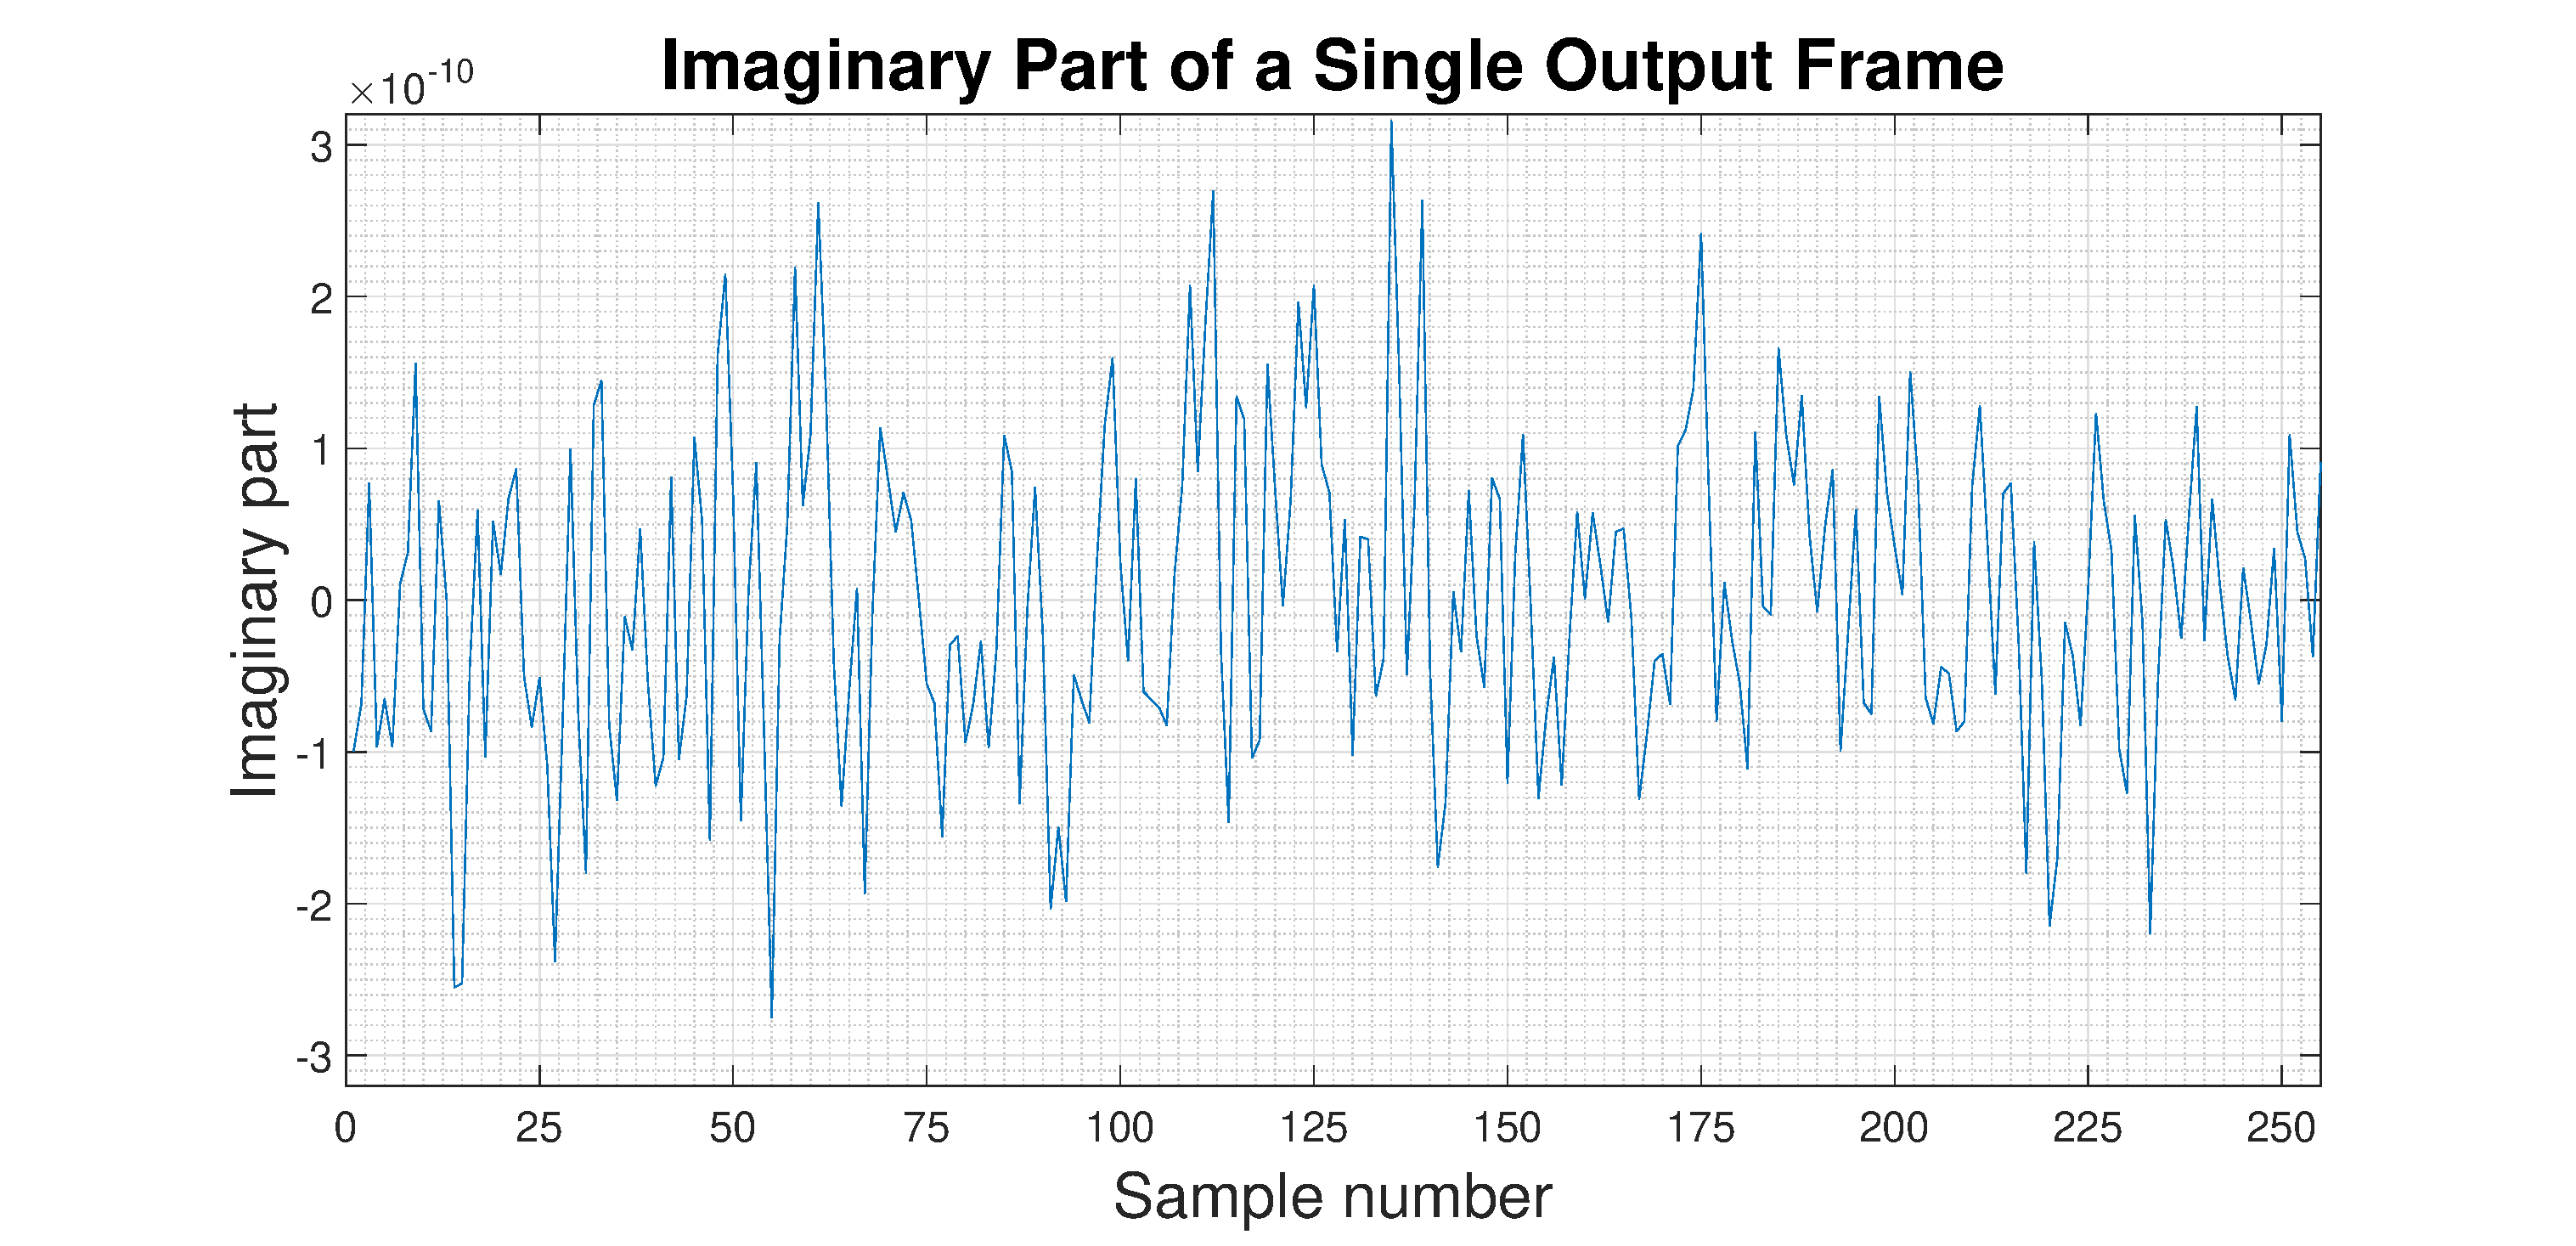
\includegraphics[width=\columnwidth]{y_imaginary}
  	\caption{Imaginary part of complex number returned when {\tt ifft} function is called}
	\label{fig:y_imaginary}
\end{figure}

The real part of the processed signal is sent to the output. The C code that performs this function is presented in listing \ref{lst:output}. 

\begin{listing}
\begin{minted}[fontsize=\scriptsize]{C}
// take inverse FFT
ifft(FFTLEN, Y);

for(i = 0; i < FFTLEN; i++){
    // send real part of Y to the output
    outframe[i] = real(Y[i]);
}	
\end{minted}
\caption{Computation of output} 
\label{lst:output}
\end{listing}

\subsection{Analysis of Performance}\label{sec:analysis_of_performance}
The speech enhancer implemented above performs simple noise filtering. The background noise in the output is significantly lower than that in the input. \textbf{We notice that the amount of noise in the system is highly dependent on the value of $\alpha$.} Figure \ref{fig:g_w_alpha_1} shows the value of $g(\omega)$ with $\alpha=1$. 

\begin{figure}[H]
	\centering
	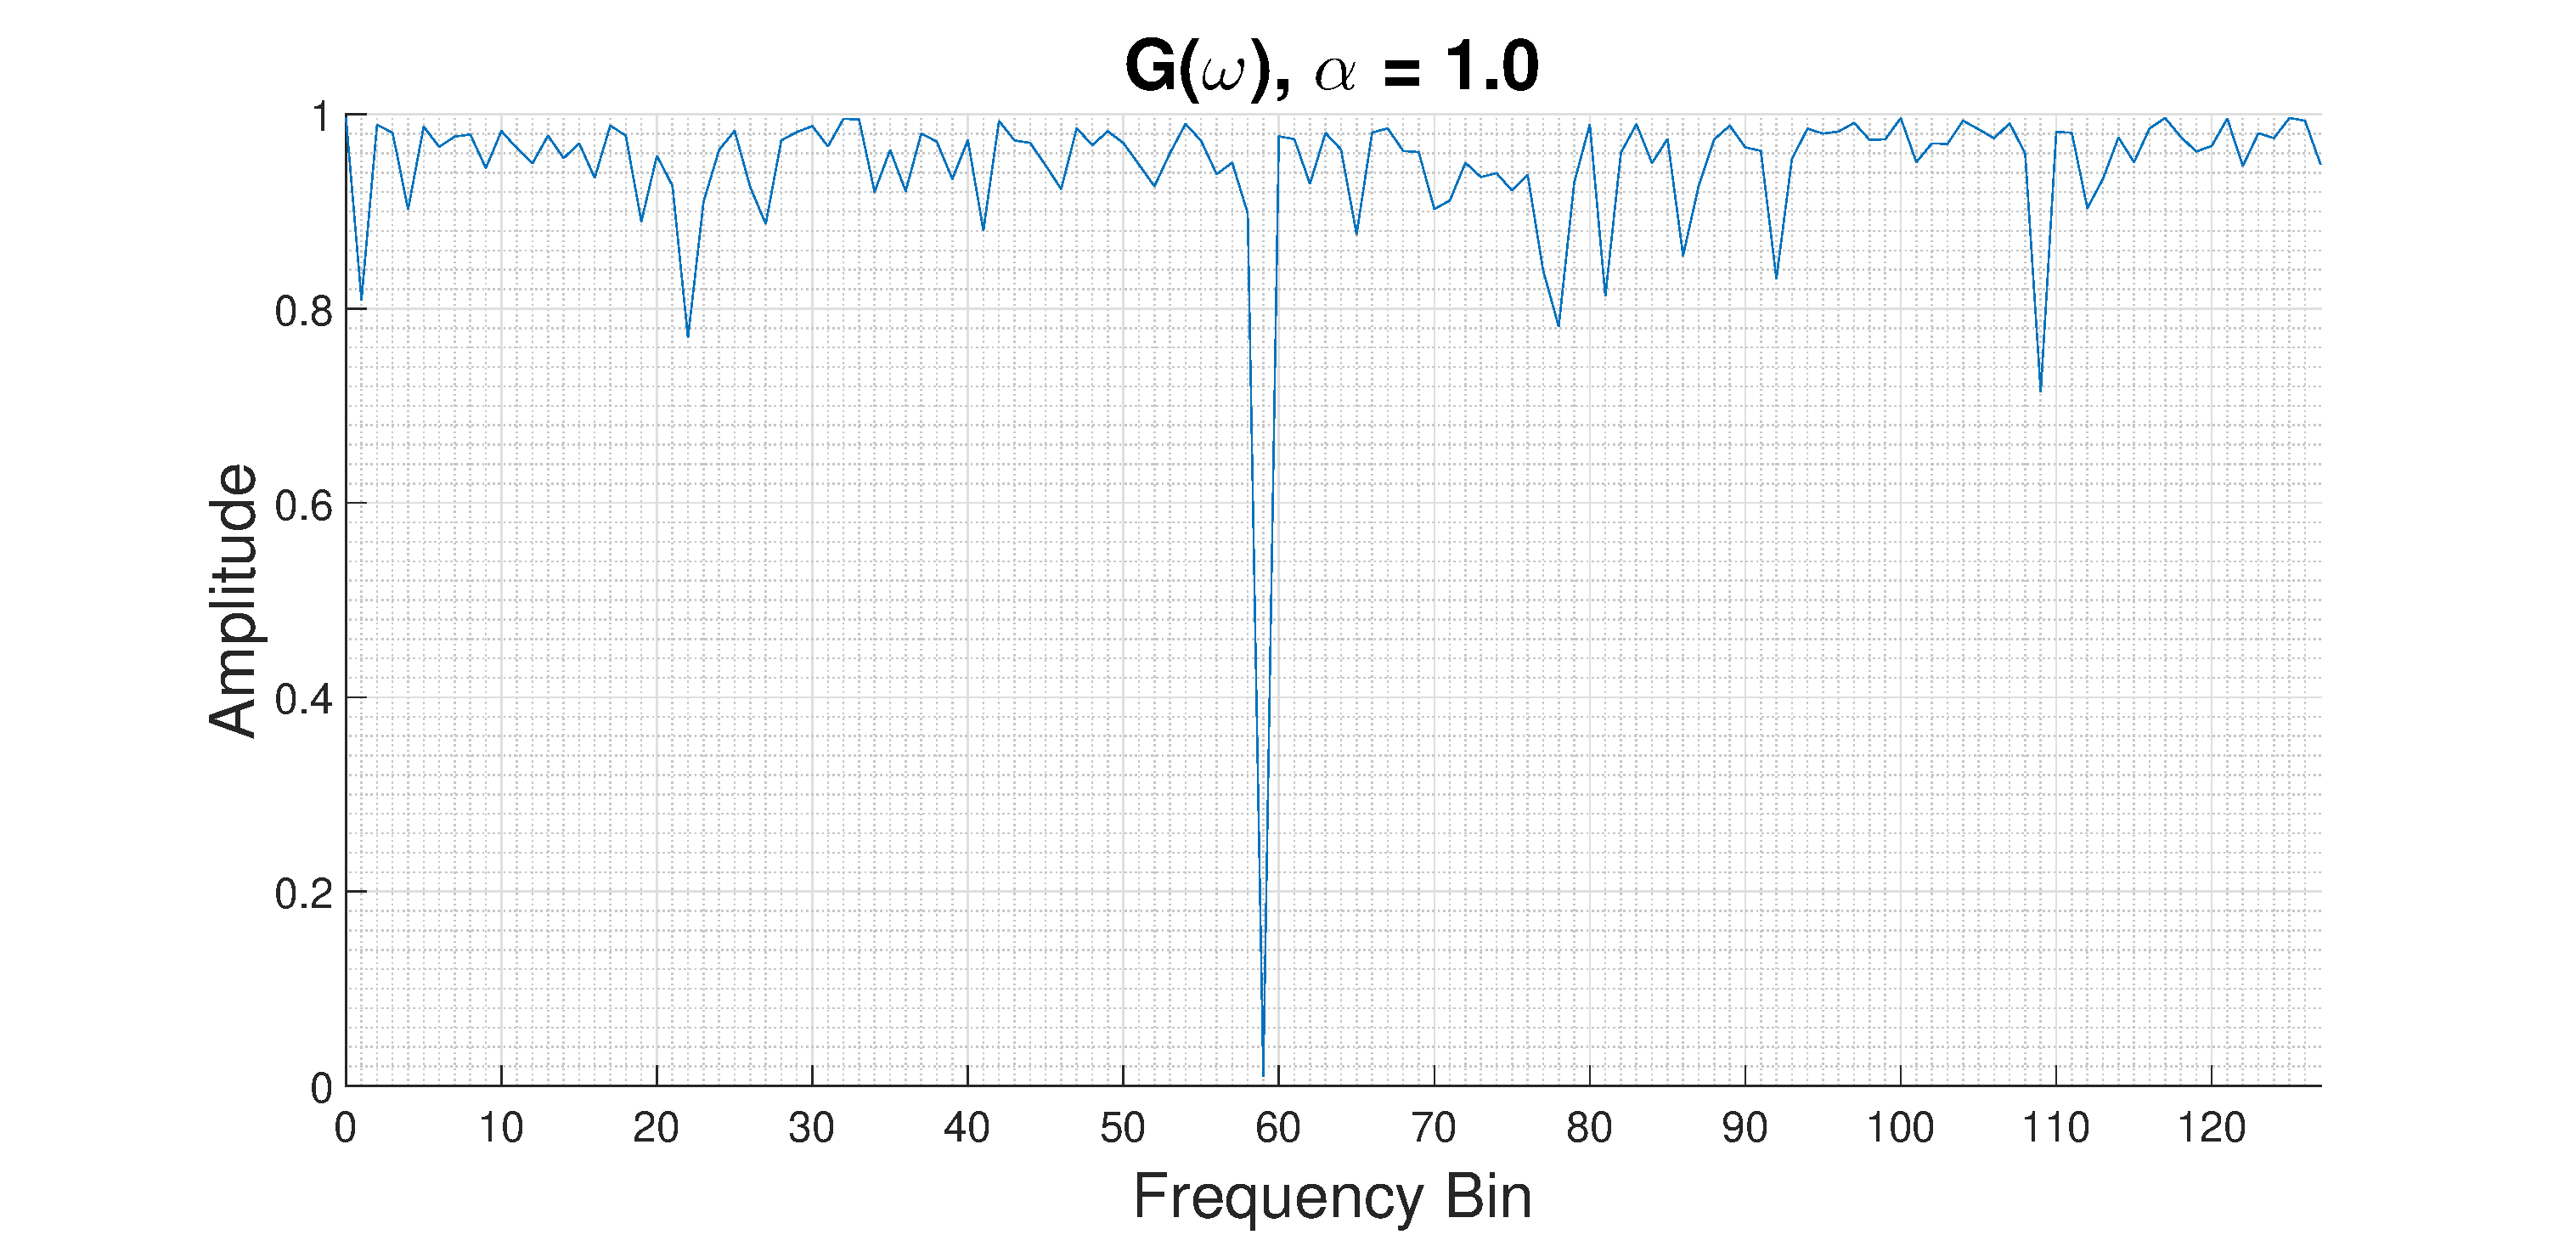
\includegraphics[width=\columnwidth]{g_w_alpha_1}
  	\caption{Value of $g(\omega)$ when $\alpha=1$}
	\label{fig:g_w_alpha_1}
\end{figure}

Figure \ref{fig:g_w_alpha_2} shows the value of $g(\omega)$ with $\alpha=5$. \textbf{Having $g(\omega)$ heavily dependent on $\alpha$ is not desirable as the system is not adaptable to different algorithms}. Secondly, notice that with $\alpha = 1$, the effect of the filtering process is not significant; as mentioned the algorithm severely underestimates the amount of noise and a large $\alpha$ is necessary to compensate for this.

\begin{figure}[H]
	\centering
    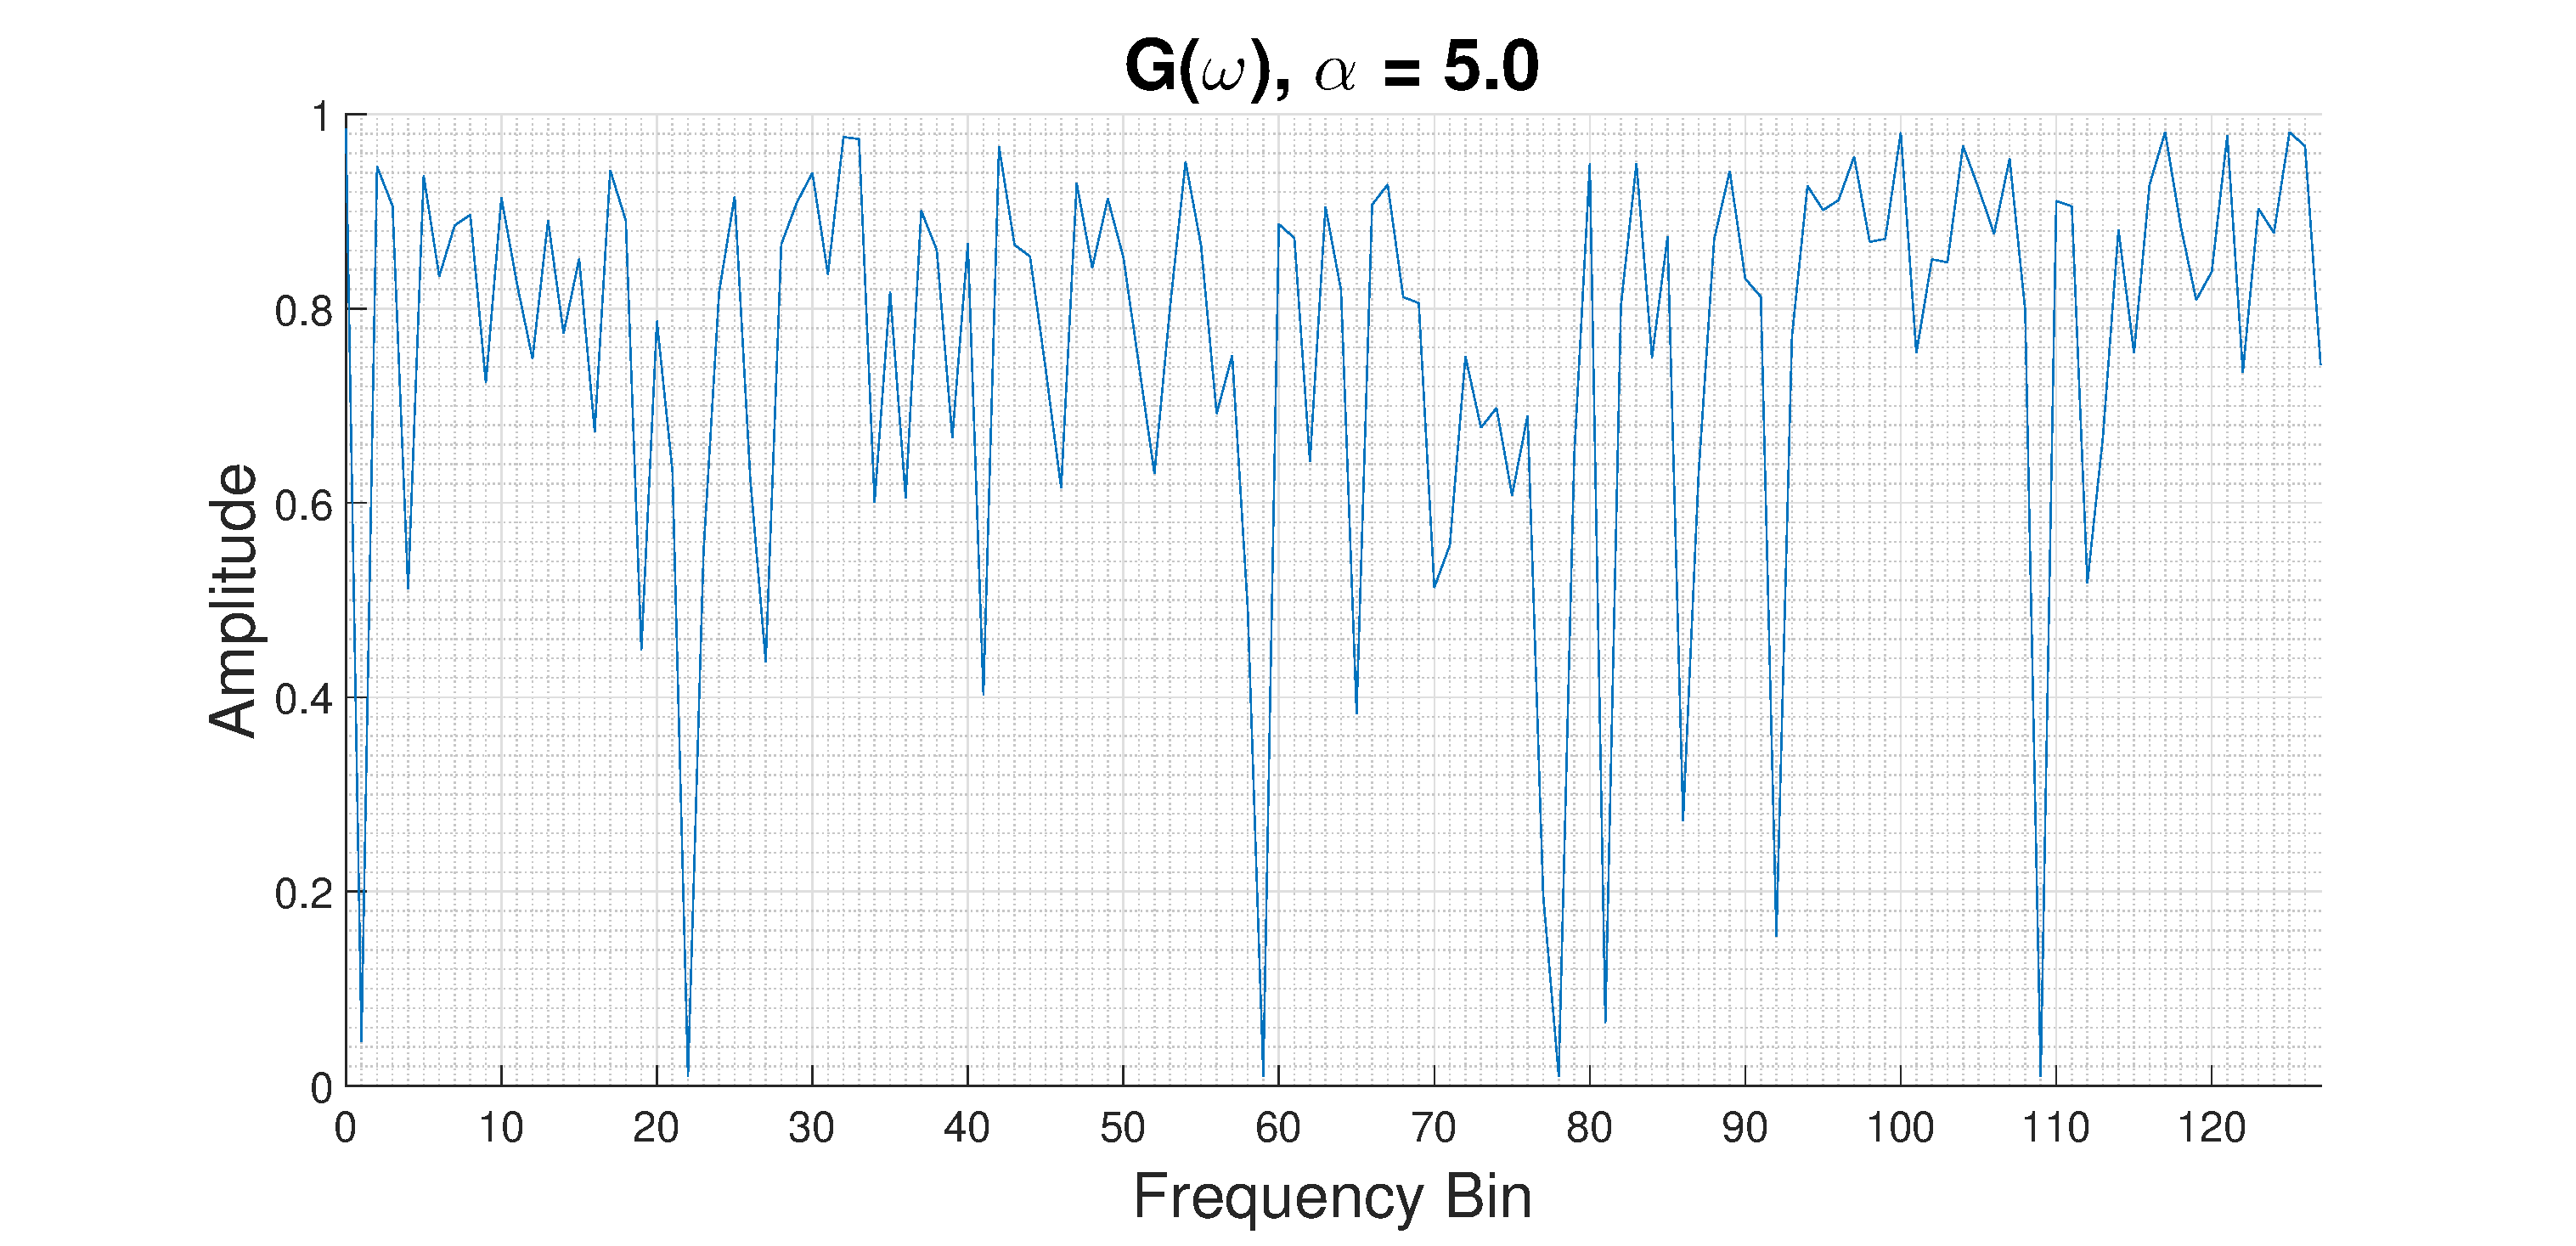
\includegraphics[width=\columnwidth]{g_w_alpha_5}
  	\caption{Value of $g(\omega)$ when $\alpha=5$}
	\label{fig:g_w_alpha_2}
\end{figure}	


Secondly, the output has an artifact referred to as musical noise. Figure \ref{fig:musical_noise_graph} shows the magnitude spectrum of adjacent frames and it is clear that at certain frequency bins, there are very drastic changes in magnitude. This is most notable at frequency bin number 40 and 50. The large peaks that only occur for short instances of time, especially when the speaker is paused, produce the musical noise that is heard. The larger the peaks, the worse the musical noise effect. The enhancements proposed in section \ref{sec:enhancements} will address both these problems. 

\begin{figure}[H]
	\centering
	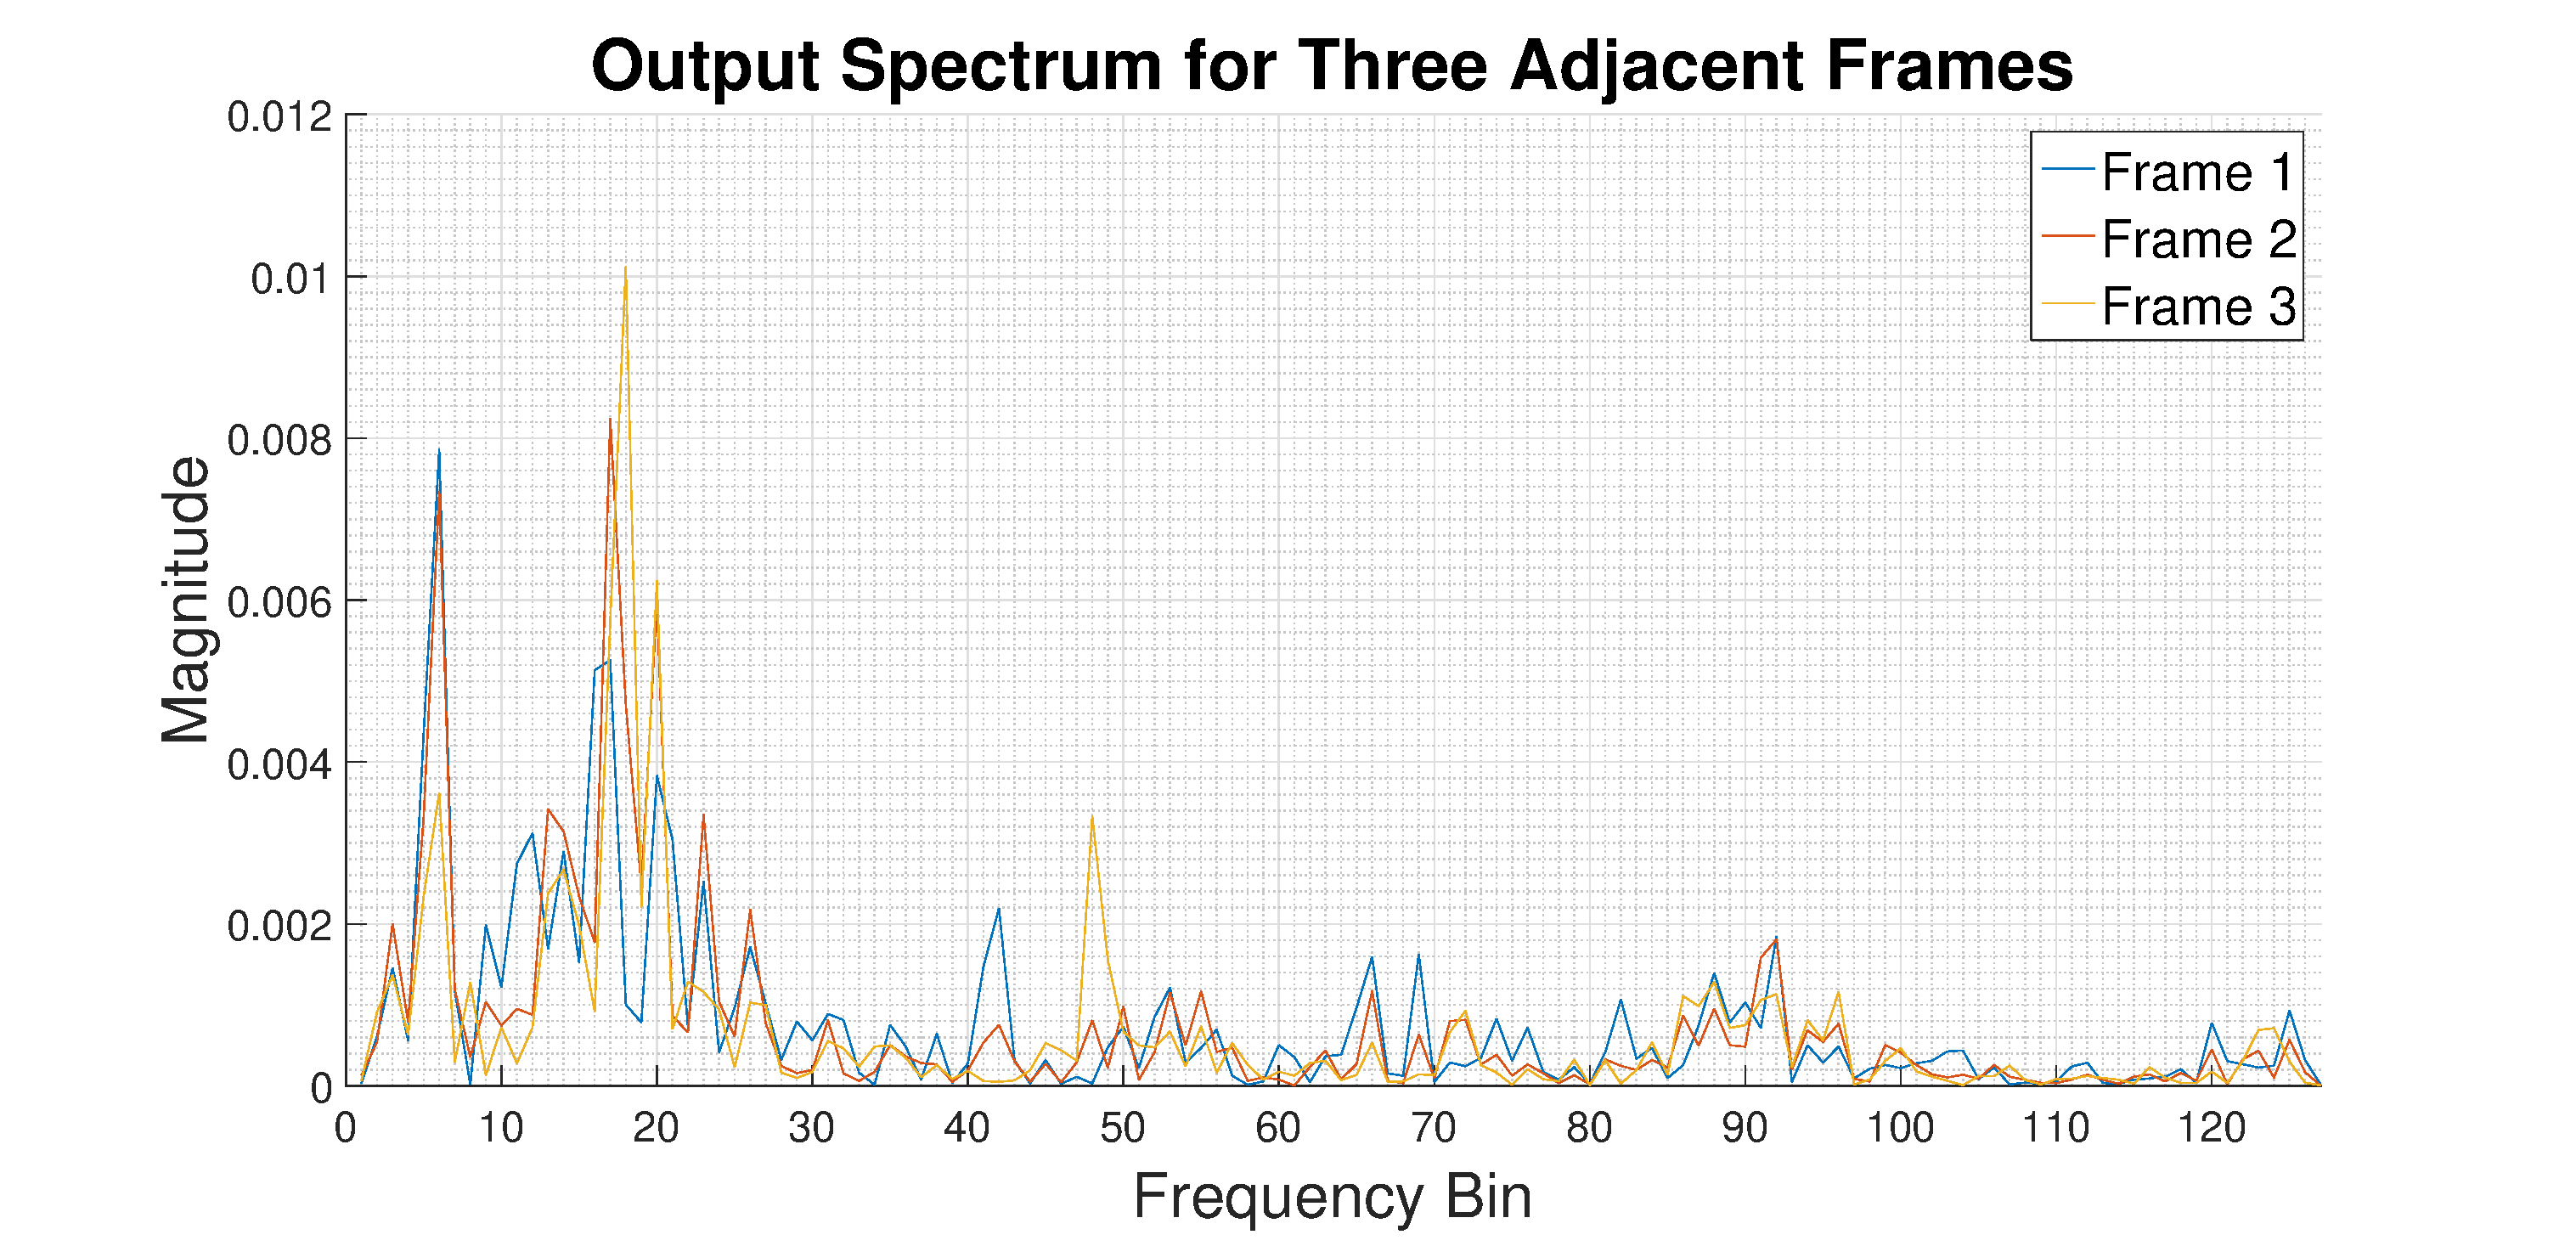
\includegraphics[width=\columnwidth]{Y_3_adjacent}
  	\caption{Musical noise artifacts due to isolated short-lived spectral peaks in adjacent output frames}
	\label{fig:musical_noise_graph}
\end{figure}

\section{Enhancements}\label{sec:enhancements}

As discussed in section \ref{sec:analysis_of_performance}, the implemented algorithm is not ideal and can be significantly improved. In this section, multiple enhancements are considered. Note that although some enhancements works well, some have an adverse effect on the output. All enhancements are carefully considered before a final selection is made. 

\subsection{Enhancement 1: Low Pass Filtering}\label{sec:enhance_1}

The first enhancement requires low-pass filtering the magnitude spectrum of the input signal. \textbf{It is of critical importance to note that the filtering is performed on the magnitude spectrum of the current frame. The filtering is not performed on the time-domain signal; the first step of the speech enhancement process is still to take the FFT.} As discussed in section \ref{sec:analysis_of_performance}, the filtered signal has a significant amount of musical noise. The musical noise comes from the fact that the magnitude spectrum is evolving very rapidly. The fast evolution causes large peaks to occur for short periods of time; this is especially true due to the random nature of the noise. Although over a large period of the time, the averaged noise has a regular magnitude spectrum, over a short period of time, the magnitude spectrum is changing rapidly.

These large peaks correspond to tones in the time-domain. The human ear is extremely sensitive to these tones and the output sounds distorted. \textbf{The evolution of the magnitude spectrum can be slowed down if it is passed through a low-pass filter. Again, it is extremely important to note that the low-pass filter will have the same effect on all frequency bins; the evolution of all frequency bins is being slowed as a function of time.} Equation (\ref{eq:lp_filter}) shows how low-pass filtering is implemented on an arbitrary frequency bin, $f_{1}$.

\begin{align}
    P_{f_{1}}(n) = (1 - e^{-\frac{T}{\tau_{s}}})*|X_{f_{1}}(n)| + e^{-\frac{T}{\tau_{s}}}*P_{f_{1}}(n-1)\label{eq:lp_filter}
\end{align}

In equation (\ref{eq:lp_filter}), $\tau$ is the time constant of the low-pass filter. Taking the z-transform of equation (\ref{eq:lp_filter}), the transfer function stated in equation (\ref{eq:lp_tf}) is obtained. 

\begin{align}
    H_{f_{1}}(z) = \frac{P_{f_{1}}(z)}{X_{f_{1}}(z)} = \frac{1 - e^{-\frac{T}{\tau_{s}}}}{1-e^{-\frac{T}{\tau_{s}}}z^{-1}}\label{eq:lp_tf}
\end{align}

\textbf{It is clear that the low-pass filtering is implemented through a first-order IIR filter.} The filter has a zero at the origin and a pole at $e^{-\frac{T}{\tau}}$. $\tau$ is a critical parameter that will determine the position of the pole in the z-domain; i.e. it will determine the cut-off frequency of the low-pass filter. It is important to note that the filter is going to be stable regardless of the value of $\tau$ as $e^{-\frac{T}{\tau}}$ is always less than $1$ and thus the pole is always within the unit circle. The value of $\tau$ will depend on the corner frequency that is desired. Equation (\ref{eq:lp_cf}) shows the relationship between the corner frequency of the filter and the value of $\tau$. Note that in equation (\ref{eq:lp_cf}), $k = e^{-\frac{T}{\tau_{s}}}$

\begin{align}
    \omega_{c} = cos^{-1}\Big(\frac{1+k^{2}-2(1-k^{2})}{2k}\Big)\label{eq:lp_cf}
\end{align}

At this point in time, the significance of $\tau$ is hard to understand. In addition, the idea of corner frequency is not as straight forward as the filtering process is applied to the frequency domain signal. To visualise the effects of $\tau$ on the magnitude spectrum, the "impulse" response of the filter is studied. In figure \ref{fig:lp_impulse_1}, an input $X_{f}(0)$ is sent to the filter. Note that the filter has the same effect on all frequency bins and thus only 40, out of 256, frequency bins have been graphed. The evolution of $P_{f}$ is studied for $n=1$ and $n=2$.

\begin{figure}[H]
	\centering
	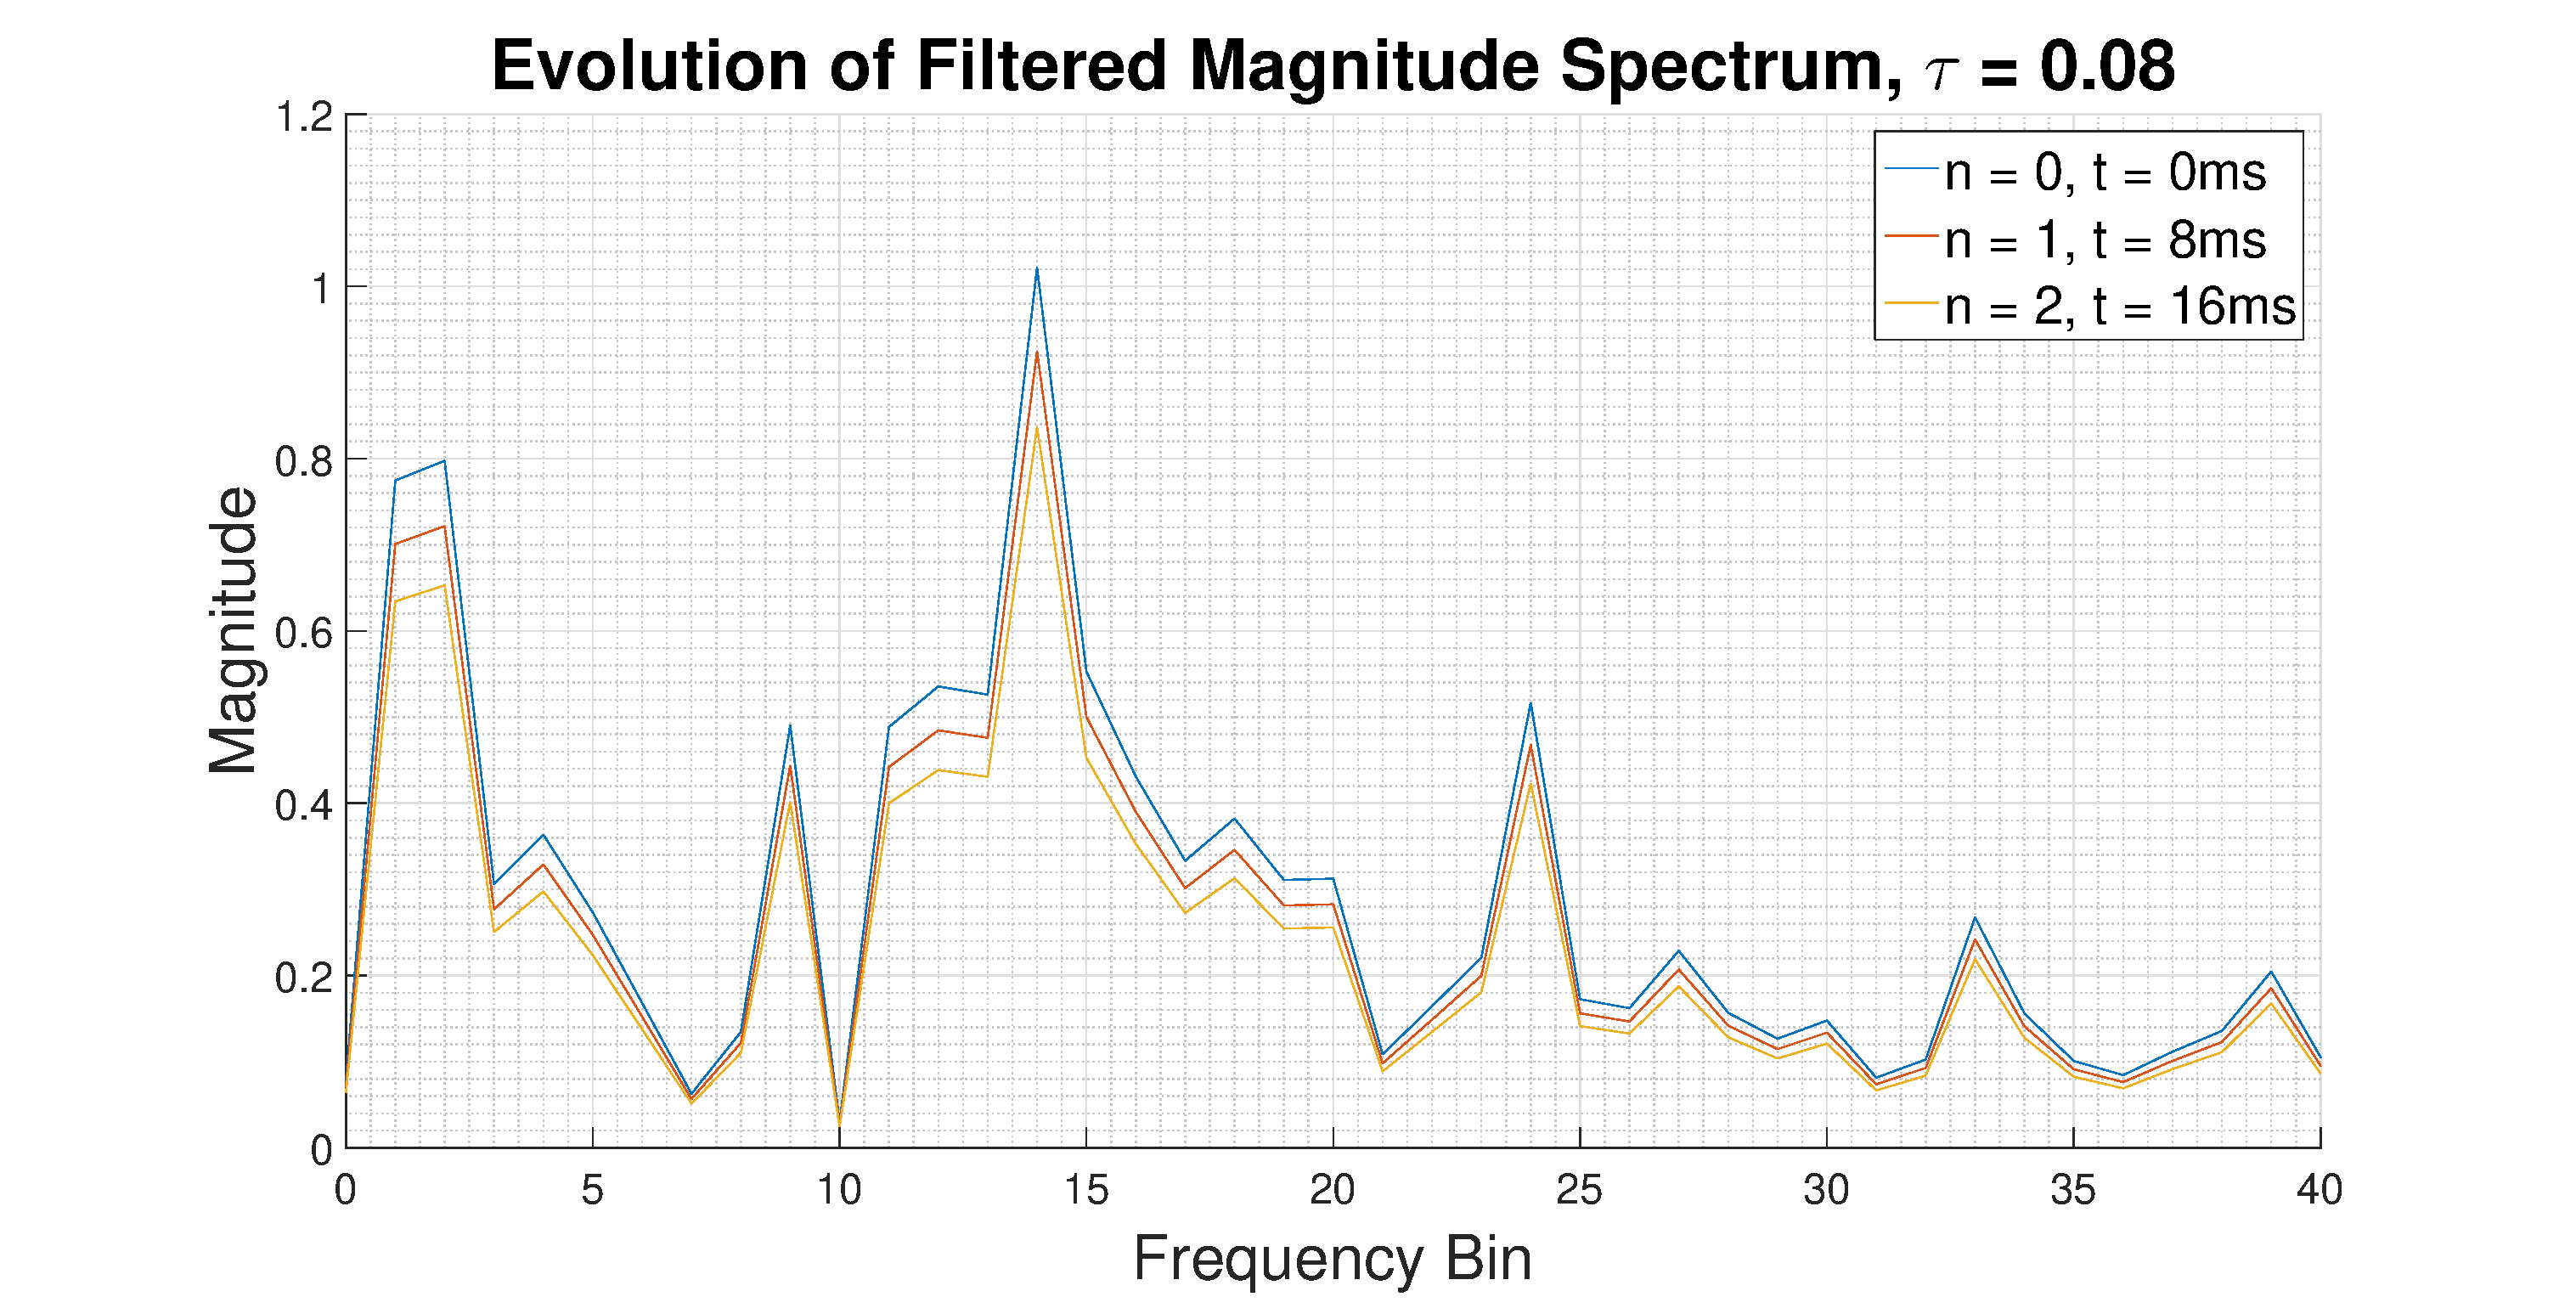
\includegraphics[width=\columnwidth]{X_filt_tau_008}
  	\caption{Low pass filter "impulse" response with $\tau=80ms$}
	\label{fig:lp_impulse_1}
\end{figure}


It is clear that having a large time constant such as $\tau=80ms$ will slow down the evolution of the magnitude spectrum to a great extent. It will take approximately $300ms$ for the frequency domain signal to be attenuated to the point that it is no longer has a significant effect on the output. \textbf{Although it is desirable to slow down the rate at which the magnitude spectrum is changing, introducing a large amount of memory into the system is not desirable.} Speech signals themselves change quite rapidly. The average person says about 130 words per minute which translates to about 1 word every $500ms$. Having a time constant of $80ms$ is extremely high. Using $\tau=20ms$ will provide a balanced trade-off between reducing the musical noise and ensuring that the magnitude spectrum is flexible enough to fully represent the changing speech signal. 

\begin{figure}[H]
	\centering
	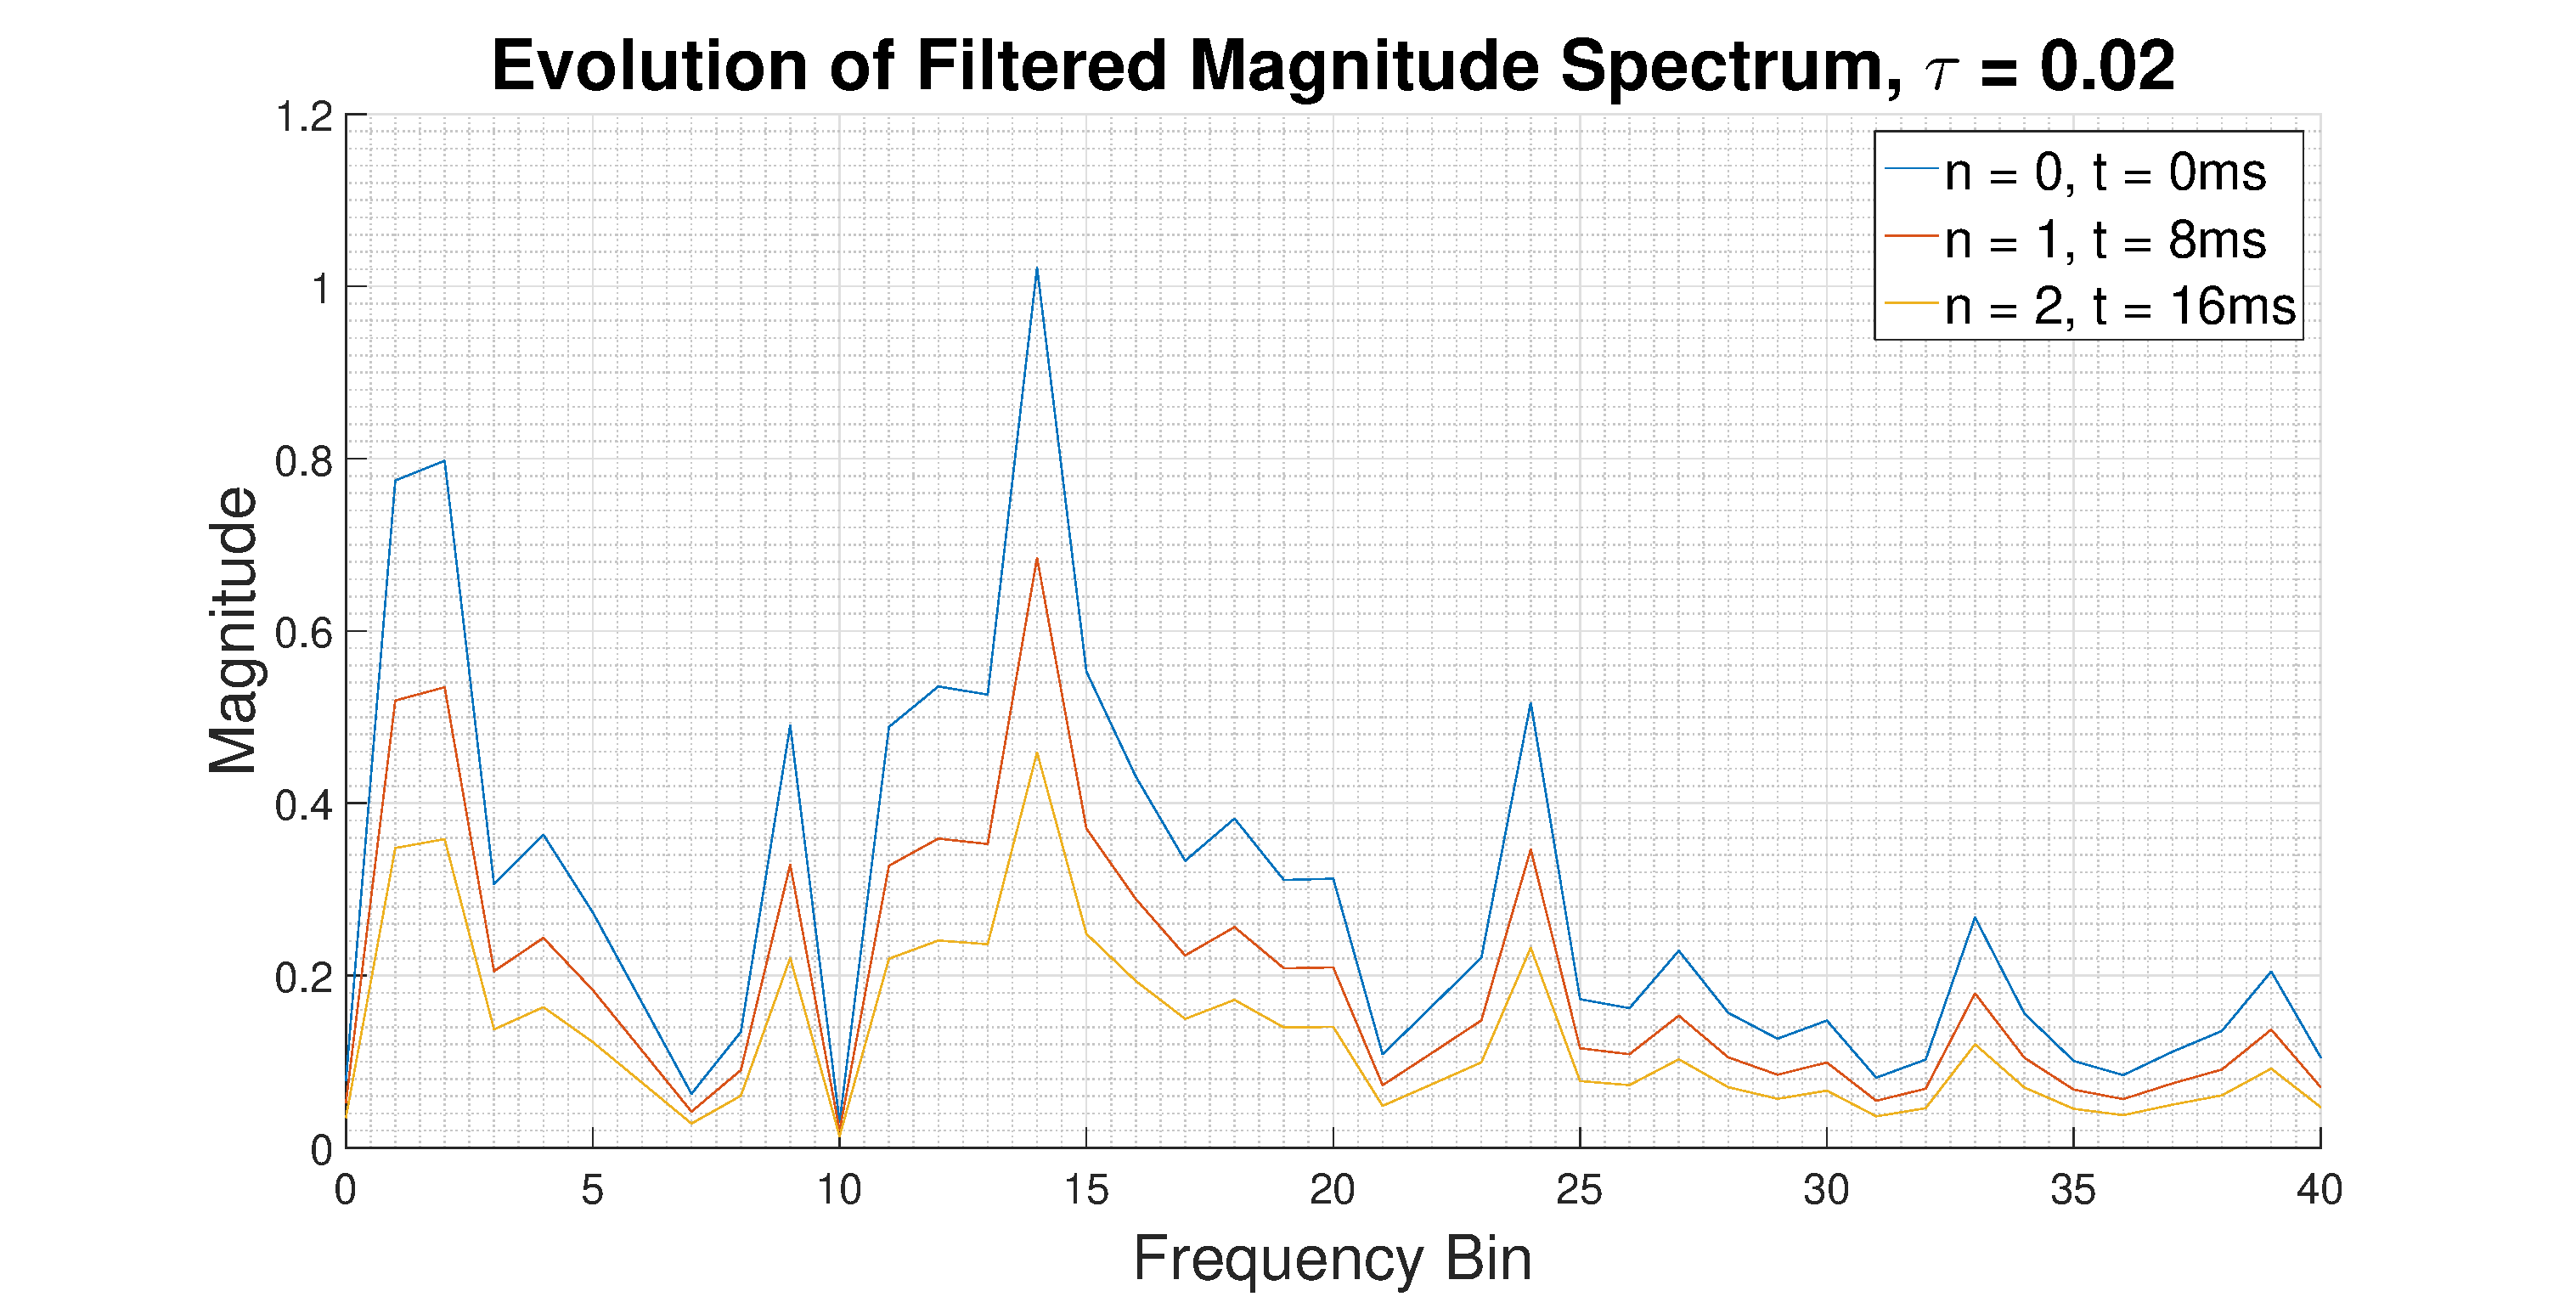
\includegraphics[width=\columnwidth]{X_filt_tau_002}
  	\caption{Low pass filter "impulse" response with $\tau=20ms$}
	\label{fig:musical_noise_graph_2}
\end{figure}

Next, the designed low-pass filter is implemented in C. The code that performs the low-pass filtering process is presented in listing \ref{lst:lp}. Note that an additional buffer is not required to store the previous value of $P(\omega)$

\begin{listing}[H]
\begin{minted}[fontsize=\scriptsize]{C}
for(i = 0; i < FFTLEN; i++){
    // compute output of first order IIR filter
    P_W[i] = (1-K_SIG)*cabs_X[i] + K_SIG*P_W[i];
}	
\end{minted}
\caption{C code used to low-pass filter magnitude spectrum} 
\label{lst:lp}
\end{listing}

The enhancement has a significant impact on reducing the amount of musical noise in the system. As expected, with $\tau = 80ms$, the signal was extremely distorted; $\tau = 20ms$ provided a cleaner output.

\textbf{It would be ideal if the source of the frequencies at which the musical noise is occurring were known. The change in magnitude spectrum could be slowed down at those particular frequencies.}

\subsection{Enhancement 2: Low-Pass Filtering in Power Domain}
The low-pass filtering process in the power domain can be mathematically expressed as in equation (\ref{eq:lp_power}).

\begin{align}
    P_{f_{1}}^{2}(n) = (1 - e^{-\frac{T}{\tau_{sp}}})*|X_{f_{1}}(n)|^{2} + e^{-\frac{T}{\tau_{sp}}}*P_{f_{1}}^{2}(n-1)\label{eq:lp_power}
\end{align}

Again the objective is similar to the objective discussed in section \ref{sec:enhance_1}, to slow down the evolution of the magnitude spectrum. Both enhancement 1 and 2 achieve this objective in slightly different ways. The C code necessary to low-pass filter in the power domain is presented in listing \ref{lst:lp_power}.

\begin{listing}[H]
\begin{minted}[fontsize=\scriptsize]{C}
for(i = 0; i < FFTLEN; i++){
    // filter in the power domain
    P_W_POW[i] = ((1-K_SIG_POWER)*(cabs_X[i])^2 
                 + K_SIG_POWER*(P_W_POW[i])^2)^(1/2);
}	
\end{minted}
\caption{C code used to low-pass filter magnitude spectrum} 
\label{lst:lp_power}
\end{listing}

Initially, it was conjectured that low-pass filtering in the power domain would produce better results. Squaring a signal is a non-linear process. The difference between the value of the magnitude of $X_{f_{1}}$ at $n=0$ and the magnitude of  $X_{f_{1}}$ at $n=1$ are scaled non-linearly. As such, the filter should have better resolution at identifying frequencies that are changing rapidly. However, as discussed in section \ref{sec:enhance_1}, a good filter is one that balances the trade off between reducing musical noise and ensuring the system is flexible enough to deal with speech signal, which are inherently fast-changing. The balanced trade-off could not be achieved with enhancement 2 and thus, the final algorithm will filter in the magnitude domain rather than in the power domain.

\subsection{Enhancement 3: Low-Pass Filter Noise Estimate}\label{sec:noise_filter}

\textbf{As discussed in section \ref{sec:enhance_1}, the low-pass filter acts equally on all frequencies. This is not ideal; frequencies at which there is a large amount of musical noise should be slowed down to a greater extent, i.e filtered with a larger value of $\tau$, as compared to frequency bins with a small amount of musical noise.} It is extremely hard to identify the source of the musical noise however, frequency selective low-pass filtering can be implemented indirectly. By filtering the noise, a frequency selective filter that slows down the rate of change of different frequency bins can be implemented. The filter is mathematically expressed in equation (\ref{eq:noise_filt}). Note the low-pass filter that acts on the noise has a unique time constant, namely, $\tau_{s}$

\begin{align}
    M_{f_{1}}(n) = (1 - e^{-\frac{T}{\tau_{n}}})*|N_{f_{1}}(n)| + e^{-\frac{T}{\tau_{n}}}*M_{f_{1}}(n-1)\label{eq:noise_filt}
\end{align}

The C code required to implement enhancement 3 is presented in listing \ref{lst:enhance3}. 

\begin{listing}[H]
\begin{minted}[fontsize=\scriptsize]{C}
for (i=0;i<FFTLEN;i++){
    // Filter the noise to ensure no sharp changes 
    // in noise mag spec
    FILTERED_NOISE[i] = (1-K_NOISE)*M_NOISE[i] 
                        - K_NOISE*FILTERED_NOISE[i];
    
    // compute the value of g_w
    // lambda initialised to 0.01
    // alpha initialised to 5
    G_W[i] = max(lambda, 1 - alpha*FILTERED_NOISE[i]/P_W[i]);
    
    // scale the output
    // real number multiplying a complex number
    Y[i] = rmul(G_W[i], X[i]);
}
\end{minted}
\caption{Subtraction of Noise} 
\label{lst:enhance3}
\end{listing}

Firstly, observe that the minimum noise buffers still hold the value of the unfiltered noise estimate and not the value of the filtered noise. Equation (\ref{eq:noise_filt}) shows that the input to the filter is unfiltered noise and not filtered noise.

As in enhancement 2, the noise can also be filtered in the power domain. The code for this is presented in listing \ref{lst:enhance3_power}. This enhancement was particularly effective in removing musical noise. Note that $\tau_{s}$ was initialised to $80ms$. \textbf{It is desirable to slow down the rate of change of the magnitude spectrum, at frequency bins in which the noise is prevalent, by a large extent.} Filtering the magnitude spectrum is preferred to filtering in the power domain; the output obtained by filtering in the power domain was not as clear as the output obtained by filtering the magnitude spectrum. In addition, it was noticed that low-pass filtering the noise enabled the use of a smaller $\alpha$. This indicates that the estimate of noise that is obtained is more accurate.

\begin{listing}[H]
\begin{minted}[fontsize=\scriptsize]{C}
for (i=0;i<FFTLEN;i++){
    // Filter the noise to ensure no sharp changes 
    // in noise mag spec
    FILTERED_NOISE_POW[i] = ((1-K_NOISE_POW)*(M_NOISE[i])^2 
                            - K_NOISE_POW*(FILTERED_NOISE_POW[i])
                            ^2)^(1/2);
    
    // compute the value of g_w
    // lambda initialised to 0.01
    // alpha initialised to 5
    G_W[i] = max(lambda, 1 - alpha*FILTERED_NOISE_POW[i]/P_W[i]);
    
    // scale the output
    // real number multiplying a complex number
    Y[i] = rmul(G_W[i], X[i]);
}
\end{minted}
\caption{Filtering noise in the power domain} 
\label{lst:enhance3_power}
\end{listing}


\textbf{Enhancement 1 and enhancement 3 together make the algorithm extremely good at dealing with sudden changes in noise.} Most notably, without filtering, there is a sudden increase in noise when the track loops. This comes from the fact that in the time that the track is looping, the output is extremely small. These extremely small values get stored in the buffers that are meant to hold the minimum noise; the small noise estimate will cause $g(\omega)$ to be extremely close to 1. This indicates that almost no noise subtraction was performed. When the noise was filtered, this sudden increase did not occur. The value of $g(\omega)$ is now no longer dependent solely on the minimum noise. It is also dependent on the previous value of the noise.

\subsection{Enhancement 4: Computation of $g(\omega)$}
This enhancement concerns how the value of the scaling constant, $g(\omega)$ is calculated. All options available require implementing a floor that will prevent the value of $g(\omega)$ from becoming negative. In the initial algorithm, the floor was a constant $\lambda$ and it was initialised to $0.02$. In the other options available, the floor is dynamically calculated and is dependent on variables such as the input signal, the noise and the filtered signal.

All the available options were tested however the combination that produced the best result was $g(\omega) = max(\lambda, 1-\nicefrac{|M(\omega)|}{|P(\omega)|})$. This is the same combination that was used to calculate $g(\omega)$ in listing \ref{lst:enhance3}.


\subsection{Enhancement 5: Computing $g(\omega)$ in the Power Domain}
Enhancement 5 involves implementing equation (\ref{eq:enhance_5}).

\begin{align}
    (\omega) = max\bigg(\lambda, \sqrt{1-\nicefrac{|N(\omega)|^{2}}{|X(\omega)|^{2}}}\bigg)\label{eq:enhance_5}
\end{align}

This enhancementment does not have a significant effect on increasing the quality of the sound. It did however cause the sound to become extremely soft at certain points and thus it will not be used in the final algorithm.

\subsection{Enhancement 6: Over-subtraction Technique}

Enhancement 6 involves the over-subtraction technique. As discussed above the spectral subtraction process causes temporary isolated spectral peaks to occur in the output; these lead to musical noise. \textbf{Multiple other enhancements have been aimed at slowing down the rate at which the magnitude spectrum is changing; this way the peaks still occur however the rate at which they change is slow and thus the distortion is not that obvious.} However, there is another method to tackle the problem of musical noise. \textbf{This involves over-subtracting the noise estimate in order remove the spectral peaks altogether.} Simply increasing the value of $\alpha$ will achieve this. However, arbitrarily increasing $\alpha$ is not a good idea. It will indeed remove the musical noise however, the speech signal will be greatly attenuated as well. \textbf{The limitation of the current implementation is that the value of $\alpha$ as a function of frequency bins is a constant; the value of $\alpha$ at the frequencies at which the musical noise is occurring needs to be increased whereas the value of $\alpha$ at the frequencies at which there is no musical noise needs to be constant. This can be effectively achieved by using an estimate of the signal-to-noise ratio (SNR) to scale the value of $\alpha$: small values of SNR should result in a larger $\alpha$ whereas large values of SNR should result in a small $\alpha$.}

Figure \ref{fig:snr_g} shows a method of varying $\alpha$ based on the SNR using a piece-wise mapping as suggested by Berouti. 
 

\begin{figure}[h]
    \centering
    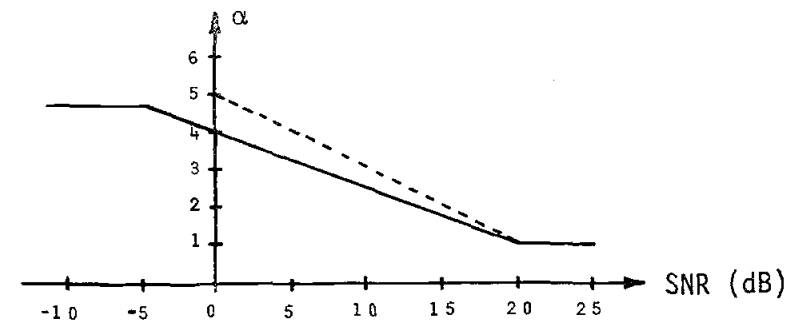
\includegraphics[width=\columnwidth]{SNR}
    \caption{Scaling of $\alpha$ using the Signal-to-Noise Ratio}
    \label{fig:snr_g}
\end{figure}

The suggested scaling of $\alpha$ as presented in figure \ref{fig:snr_g} can be represented by the piecewise function listed below.

\begin{align}
\[   \alpha = \left\{
\begin{array}{ll}\vspace{2mm}
      \alpha_0 + \frac{\alpha_0-1}{4}       &\quad SNR < -5dB \\ \vspace{2mm}
      \alpha_0 - \frac{\alpha_0-1}{20}SNR   &\quad -5dB \leq SNR\leq 20dB \\ 
      1                                     &\quad SNR > 20dB \\
\end{array} 
\right. \]
\end{align}

The C code required to represent this is presented in lisitng \ref{lst:var_alpha}.

\begin{listing}[H]
\begin{minted}[fontsize=\scriptsize]{C}
for (i=0;i<FFTLEN;i++){
    // Filter the noise to ensure no sharp changes 
    // in noise mag spec
    // noise filtering performed in mag domain,
    // not in power domain
    FILTERED_NOISE[i] = (1-K_NOISE)*M_NOISE[i] 
                        - K_NOISE*FILTERED_NOISE[i];
    
    // unfiltered noise used to calculate SNR
    // filtered noise not representative of actual 
    // signal-to-noise ratio
    SNR = 20*log( P_W[k] / M_NOISE[k] );
    
    // implement piecewise function to calculate alpha
    if(SNR < -5)
        alpha = alpha_0 + (alpha_0-1)/4;
    else if(-5 <= SNR <= 20)
        alpha = alpha_0 + SNR*(alpha_0-1)/20;
    else
        alpha = 1;

    // compute the value of g_w
    // lambda initialised to 0.01
    G_W[i] = max(lambda, 1 - alpha*FILTERED_NOISE_POW[i]/P_W[i]);
    
    // scale the output
    // real number multiplying a complex number
    Y[i] = rmul(G_W[i], X[i]);
}
   
\end{minted}
\caption{Implementing over-subtraction using the Signal-to-Noise Ratio} 
\label{lst:var_alpha}
\end{listing}

The method described above did not produce a clear output; a great number of frequency bins were hitting the floor. A slight twist is made so as to prevent this. Instead of scaling $\alpha$ directly, the value of $\alpha$ is determined by the baseline amount of noise that needs to removed. Using the baseline value of $\alpha$, $g(\omega)$ is calculated. The value of $g(\omega)$ is then scaled by the normalised SNR. The C implementation of this alternative approach is presented in listing \ref{lst:var_alpha_2}.

\begin{listing}[H]
\begin{minted}[fontsize=\scriptsize]{C}
mymax=0;
for (k=0;k<FFTLEN;k++){ 
    // unfiltered noise used to calculate SNR
    // filtered noise not representative of actual 
    // signal-to-noise ratio
	SNR[k] = 20*log( P_W[k] / M_NOISE[k] );
    
    // obtain maxmimum SNR
    // needed for normalisation
	if(SNR[k]>SNR[mymax])
		mymax = k;
}

for (i=0;i<FFTLEN;i++){
    // Filter the noise to ensure no sharp changes 
    // in noise mag spec
    // noise filtering performed in mag domain,
    // not in power domain
    FILTERED_NOISE[i] = (1-K_NOISE)*M_NOISE[i] 
                        - K_NOISE*FILTERED_NOISE[i];
                        
    // compute the value of g_w
    // lambda initialised to 0.01
    G_W[i] = max(lambda, 1 - alpha*FILTERED_NOISE_POW[i]/P_W[i]);
    
    // scale the output with normalised SNR and g_w
       // real number multiplying a complex number
    Y[i] = rmul(G_W[i]*SNR[i]/SNR[mymax], X[i]);
}
\end{minted}
\caption{Implementing over-subtraction using the Signal-to-Noise Ratio: Alternative Implementation} 
\label{lst:var_alpha_2}
\end{listing}

\subsection{Enhancement 7: Frame Lengths}
The frame length can be easily changed by changing the variable {\tt FFTLEN}. \textbf{Having a large number of points to compute the FFT is extremely desirable. The number of data points on which the FFT function is computed will determine the number of frequencies at which the FFT is evaluated. Having a large number of data points will improve the frequency resolution.} An increased frequency resolution is the main reason for oversampling the data. 

A short frame size of 128 samples was tested. The output obtained was extremely choppy. With a frame size of 256, $75\%$ of time domain samples in adjacent frames were identical. Having changed only 25\% of the time domain samples, the magnitude spectrum is still relatively similar from one frame to another. The change in the magnitude spectrum is gradual. Having a smaller frame size of 128, 50\% of the time domain samples are retained in adjacent frames. This causes the change in the magnitude spectrum to be more rapid. Discontinuities are more prevalent and thus the output is choppy. 

A longer frame size of 512 samples is tested however the output was again distorted. The output made it sound as if the speaker was speaking unnaturally slowly. Having such a large frame size causes the changes in the magnitude spectrum to be extremely gradual. The changes were so slow that it actually causes the speech to slow down as well. The output obtained was similar to the output obtained when the signal was filtered with $\tau$ = 80ms.

\subsection{Enhancement 8: Residual Noise Subtraction}

This enhancement focuses on removing musical noise artifacts from the output. S\textbf{ince the short-lived isolated spectral peaks are randomly fluctuating, they can be suppressed by taking the minimum value of the output from three adjacent frames.} A threshold, which shall be called the maximum residual noise, has to be determined. Above the threshold, a specific spectral component is assumed to be part of the speech signal. If the magnitude at the frequency bin is lower than the threshold, it is assumed to part of the noise and thus, the correct magnitude needs to be determined. There are three possible scenarios for this enhancement:
\begin{enumerate}
    \item if $|Y(\omega)| < N_R$ and the output is changing considerably from frame-to-frame then it is highly likely that this is due to noise and this is suppressed.
    \item if $|Y(\omega)| < N_R$ and the output is stationary then it is likely to be a low-energy component of the speech and it is not altered by taking the minimum over adjacent frames
    \item if $|Y(\omega)| > N_R$ then the spectral component is likely to be part of the speech and it is not necessary to take the minimum.
\end{enumerate}

The C code that implements this enhancement is provided in listing \ref{lst:min_noise}.
\begin{listing}[H]
\begin{minted}[fontsize=\scriptsize]{C}
for (k=0;k<FFTLEN;k++){ 

    // determine if spectral component is noise or part of speech
    if(cabs(Y[k]) < max_residue){
        // determine the minimum noise for three adjacent frames
        temp =  min(cabs(Y_prev[k]), 
                min(cabs(Y[k]), cabs(Y_next[k])));
    
        // assign output accordingly
        if(temp == cabs(Y_prev[k]))
            out[k] = Y_prev[k];
        else if(temp == cabs(Y[k]))
            out[k] = Y[k];
        else
            out[k] = Y_next[k];
    }
    
    // if spectral component is part of speech
    else{
        out[k] = Y[k];
    }
    
    // update buffers that hold the outputs of three frames
    Y_next[k]=Y[k];
    Y[k] = Y_prev[k];
}
\end{minted}
\caption{Residual noise subtraction} 
\label{lst:min_noise}
\end{listing}

Although extremely effective in theory, this enhancement did not improve the quality of the speech signal. It will not be used in the final algorithm.

\subsection{Enhancement 9: Shorter Window}
As mentioned in section \ref{sec:theory}, the spectral subtraction algorithm does not require the noise to be stationary. No a priori knowledge of the PDF of the noise is required. A 10 second window was initially chosen because it was assumed that the speaker would pause at least once every 10 seconds. \textbf{It is highly likely that the speaker will pause even if the window was smaller. Decreasing the size of the window will remove a great deal of memory of the system. The noise that is subtracted from the system will represent the minimum magnitude spectrum over a shorter period of time.} This is favourable. 

To implement a shorter window in C is extremely easy. The buffers are rotated more often if a shorter window is required. In the C code presented in listing \ref{lst:short_win}, the variable {\tt win\_div\_fact} is used to determine how often the buffers and rotated.

\begin{listing}[H]
\begin{minted}[fontsize=\scriptsize]{C}
// check is buffers need rotating
// win_div_fact determines how often 
if(count >= ROTATE/win_div_fact){
    // reset counter
    count = 0;
    tempPtr = M1;
    M1 = M4;
    M4 = M3;
    M3 = M2
    M2 = tempPtr;
    
    // set the buffer to FLT_MAX
    for (i = 0; i < FFTLEN; i++){
        M1[i] = FLT_MAX;
    }
}	

count++;
\end{minted}
\caption{Variable window length} 
\label{lst:short_win}
\end{listing}

Testing is performed and the results obtained are graphed in figure \ref{fig:enhance_9}.

\begin{figure}[H]
    \centering
    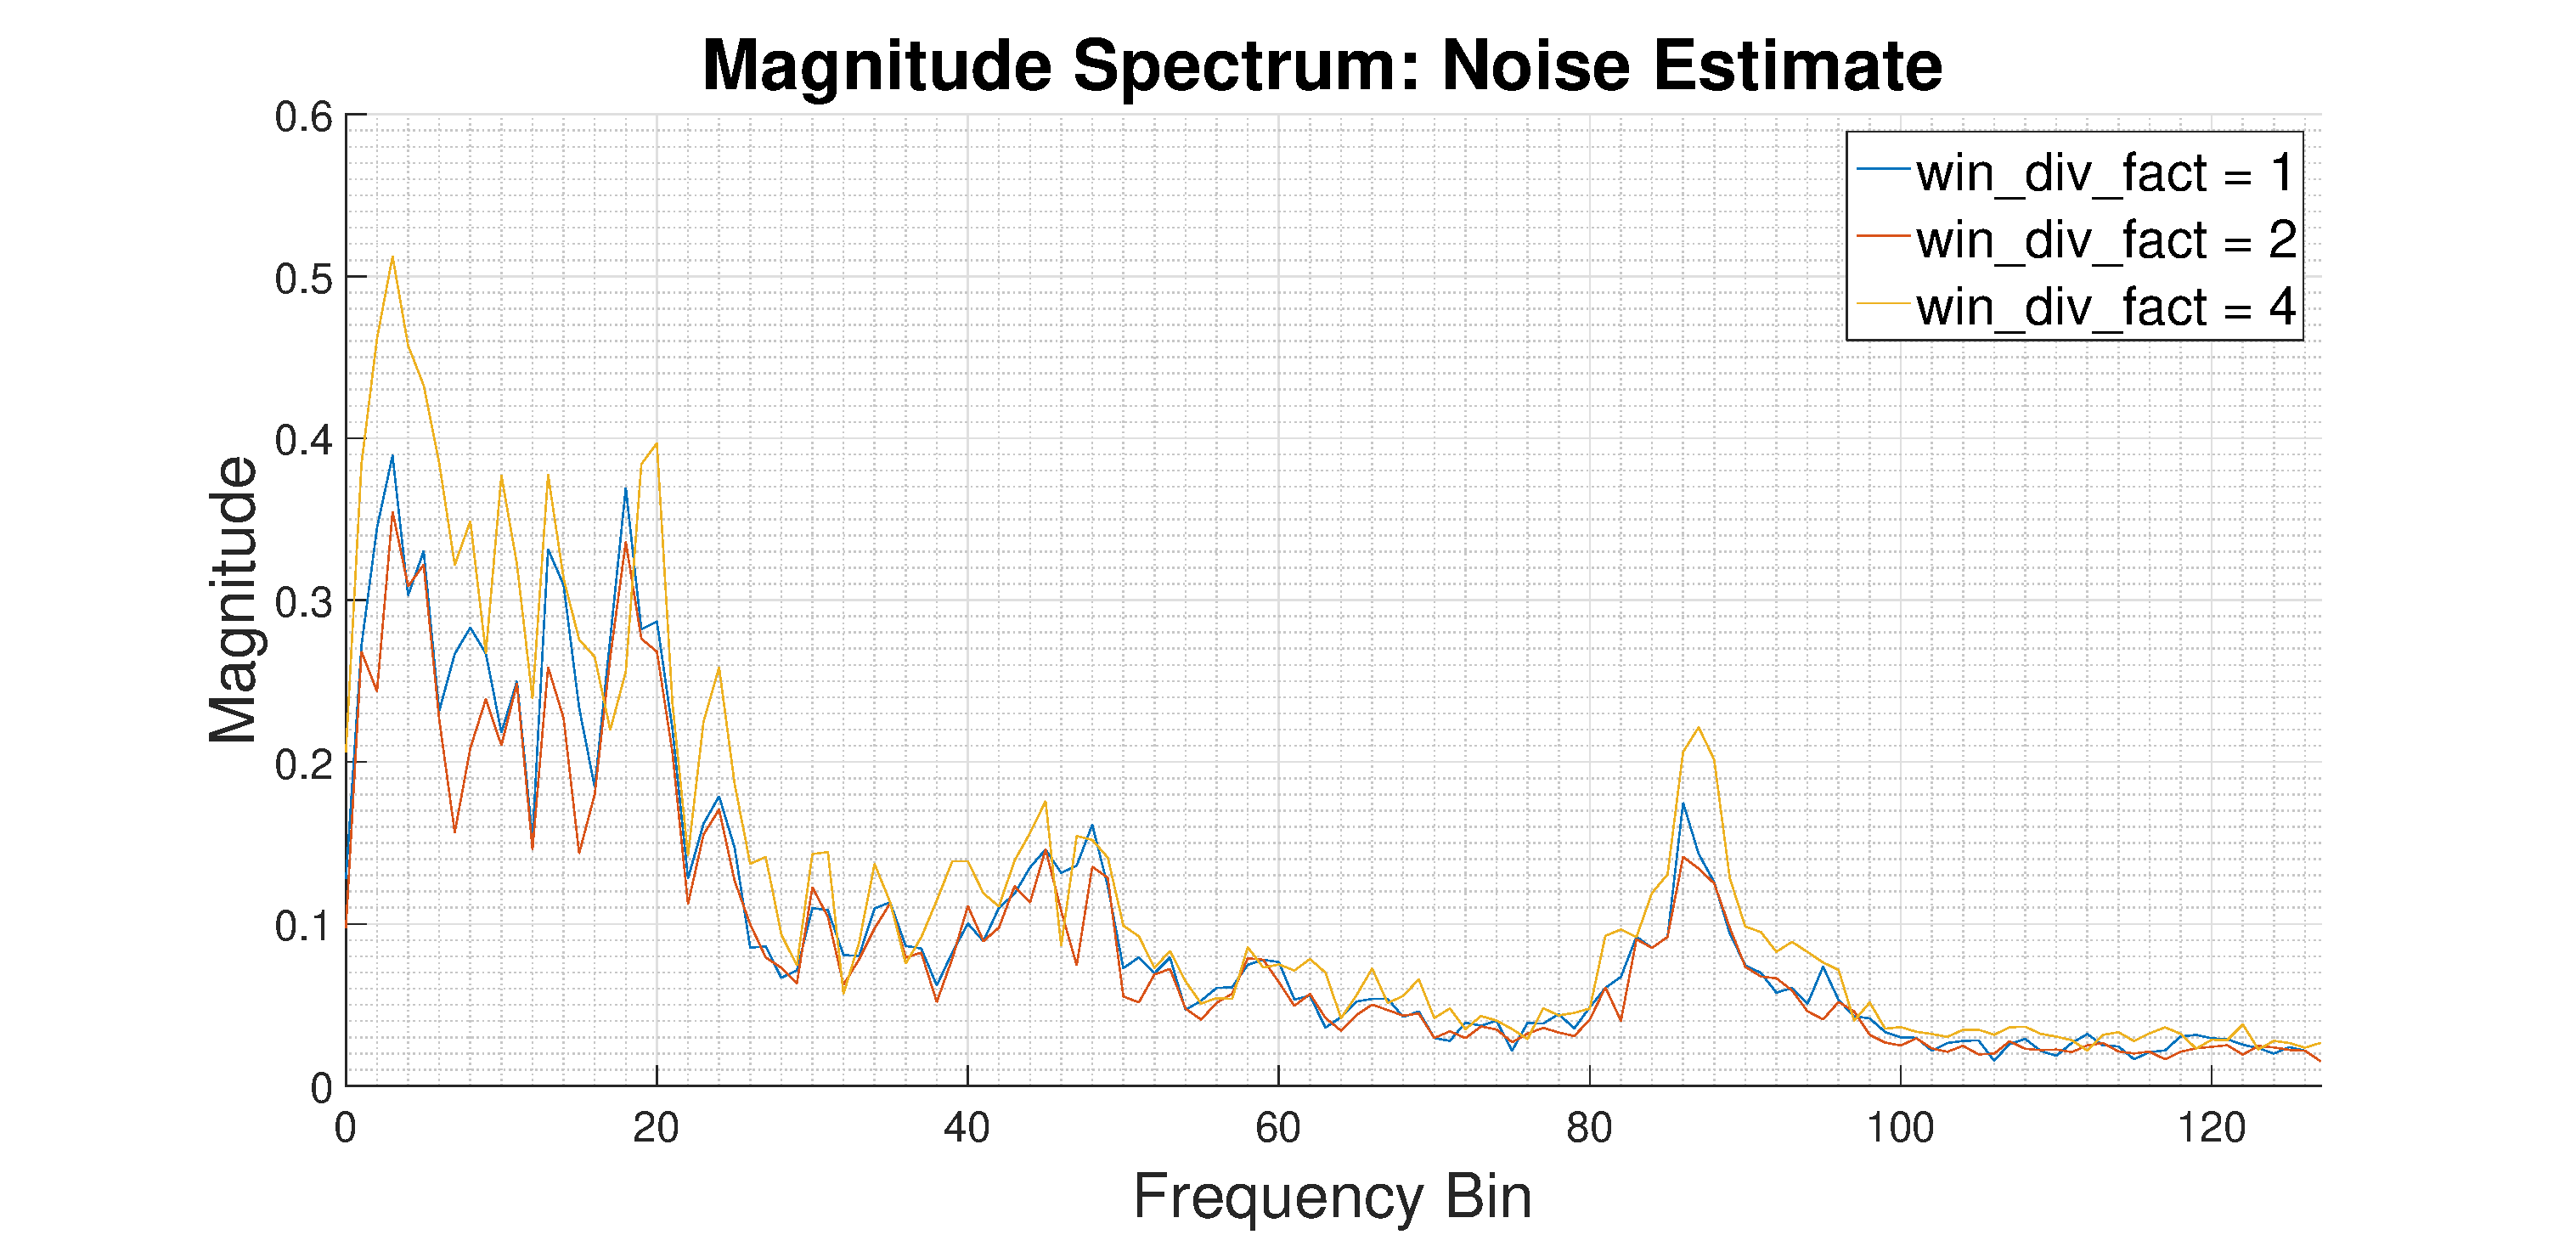
\includegraphics[width = \columnwidth]{win_div_fact}
    \caption{Effect of reducing size of averaging window}
    \label{fig:enhance_9}
\end{figure}

If {\tt win\_div\_fact} is set to 4, the noise estimate varies greatly from if {\tt win\_div\_fact} is set to 2 or 1, i.e, if noise is averaged over a 2.5 seconds window, the estimate of noise is extremely poor. The speaker does not make long enough pauses in a 2.5 second window to obtain a good noise estimate. It was however found that setting {\tt win\_div\_fact} to 2 produced the better results that setting {\tt win\_div\_fact} to 1. Again the right balance has to be found. Averaging the noise over a 5 second window provides enough time for a good noise estimate that is adaptable to noise that is non-stationary. It should be noted that throughout this assignment, the speech to which the algorithm has been optimised is constant although the nature of the noise is changing. As such, using a 5 second window is sufficient because the speaker pauses often. However, to have a robust algorithm, a longer window should still be considered. 

\section{Final Algorithm Performance}

Although many of the enhancements discussed are theoretically sound, the performance measure for a speech enhancing algorithm is rather subjective. After performing qualitative analysis it was discovered that although all of the enhancements when individually implemented suppress the noise, the best combination of enhancements are: 1 (input frame filtering in the magnitude-domain), 3 (noise frame filtering in the magnitude-domain), 4, 6b (varying $\alpha$ based on the SNR) and 9 (estimating over a shorter period).

Enhancement 1 \& 3 are used to smoothen the input and noise magnitude spectra in order to obtain an output spectrum that does not contain random isolated peaks that cause musical noise artifacts to appear in output. Although the filters aims to reduce musical noise by slowing down the evolution of the magnitude spectra, they lead to under subtraction. This in turn gives rise to an increase in musical noise. To counteract this issue, enhancement 6b uses an over-subtraction technique based on the SNR to completely eliminate a significant proportion of noise. 

In real-world applications, noise is not stationary; using a window length of 10 seconds prevents the algorithm from fully representing the non-stationarity present in the noise. Enhancement 9 decreases the window length by rotating the minimum noise buffer more often. There is a compromise between the assumption that the speaker pauses every 10 seconds and the performance of the algorithm for non-stationary noise. The final enhancement is obtained using a qualitative measure; it was found that enhancement 4e sounded cleaner than the basic calculation of $g(\omega)$ and the other suggested options.

\begin{figure}[H]
    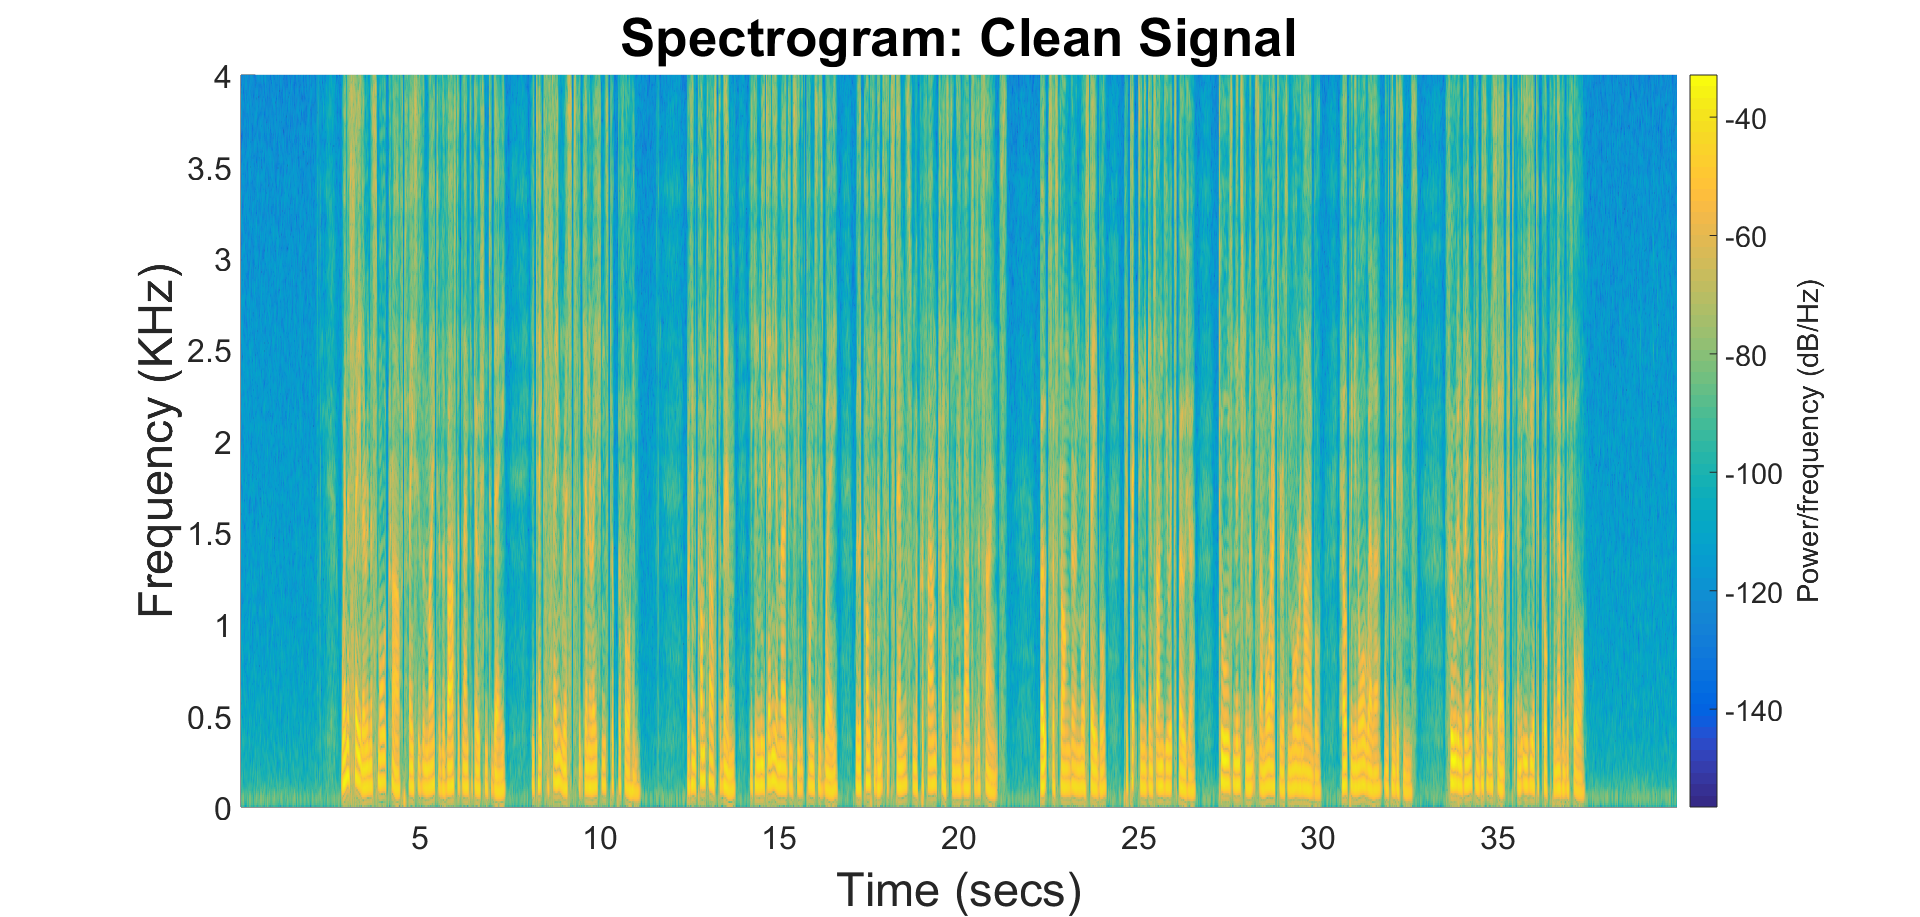
\includegraphics[width=\columnwidth]{final_clean}
    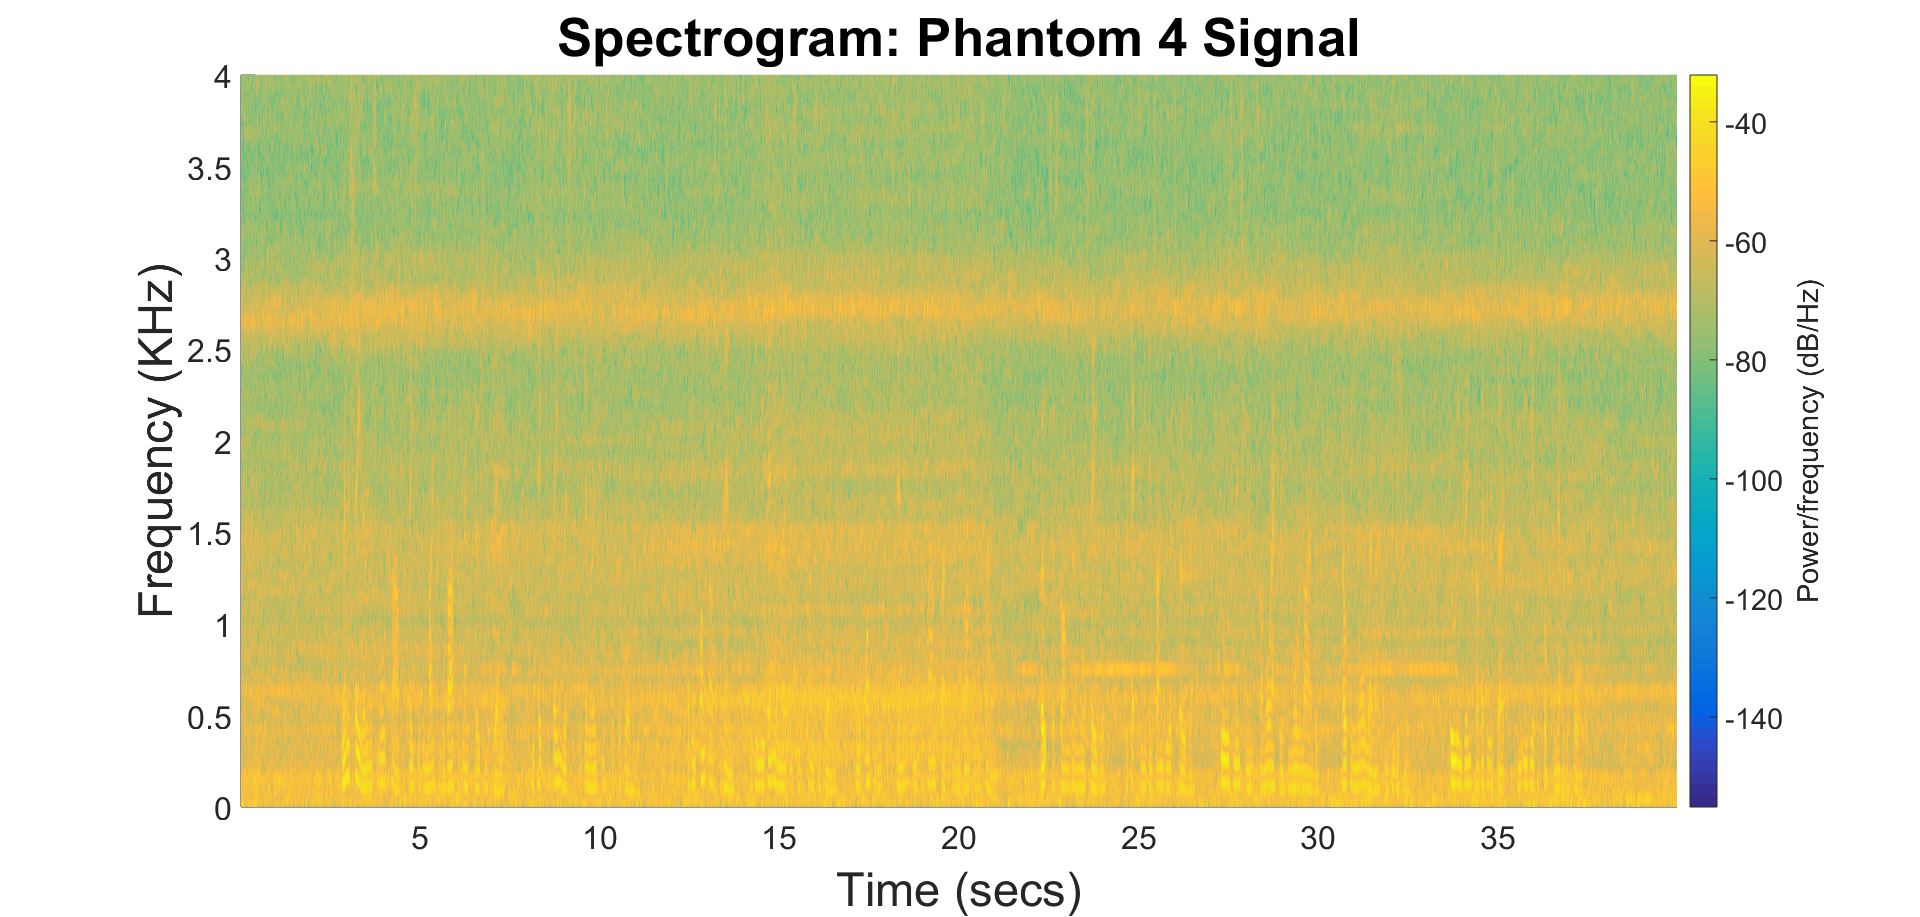
\includegraphics[width=\columnwidth]{final_ph4}
    \caption{Spectrogram of clean signal and corrupted phantom4.wav}
    \label{fig:clean}
\end{figure}

Spectral subtraction is a real-time DSP algorithm that processes speech in the frequency-domain; this means that in order to assess the performance of the final algorithm it is necessary to view the output in the frequency-domain parametrised by time - commonly referred to as a spectrogram. Figures \ref{fig:clean} and \ref{fig:dirty} shows the clean, corrupted and filtered spectrogram. Note, to assess the performance of the algorithm, a worst-case engineering approach is adopted and the corrupted signal with the largest noise variance is considered (phantom4.wav). 

\begin{figure}[H]
    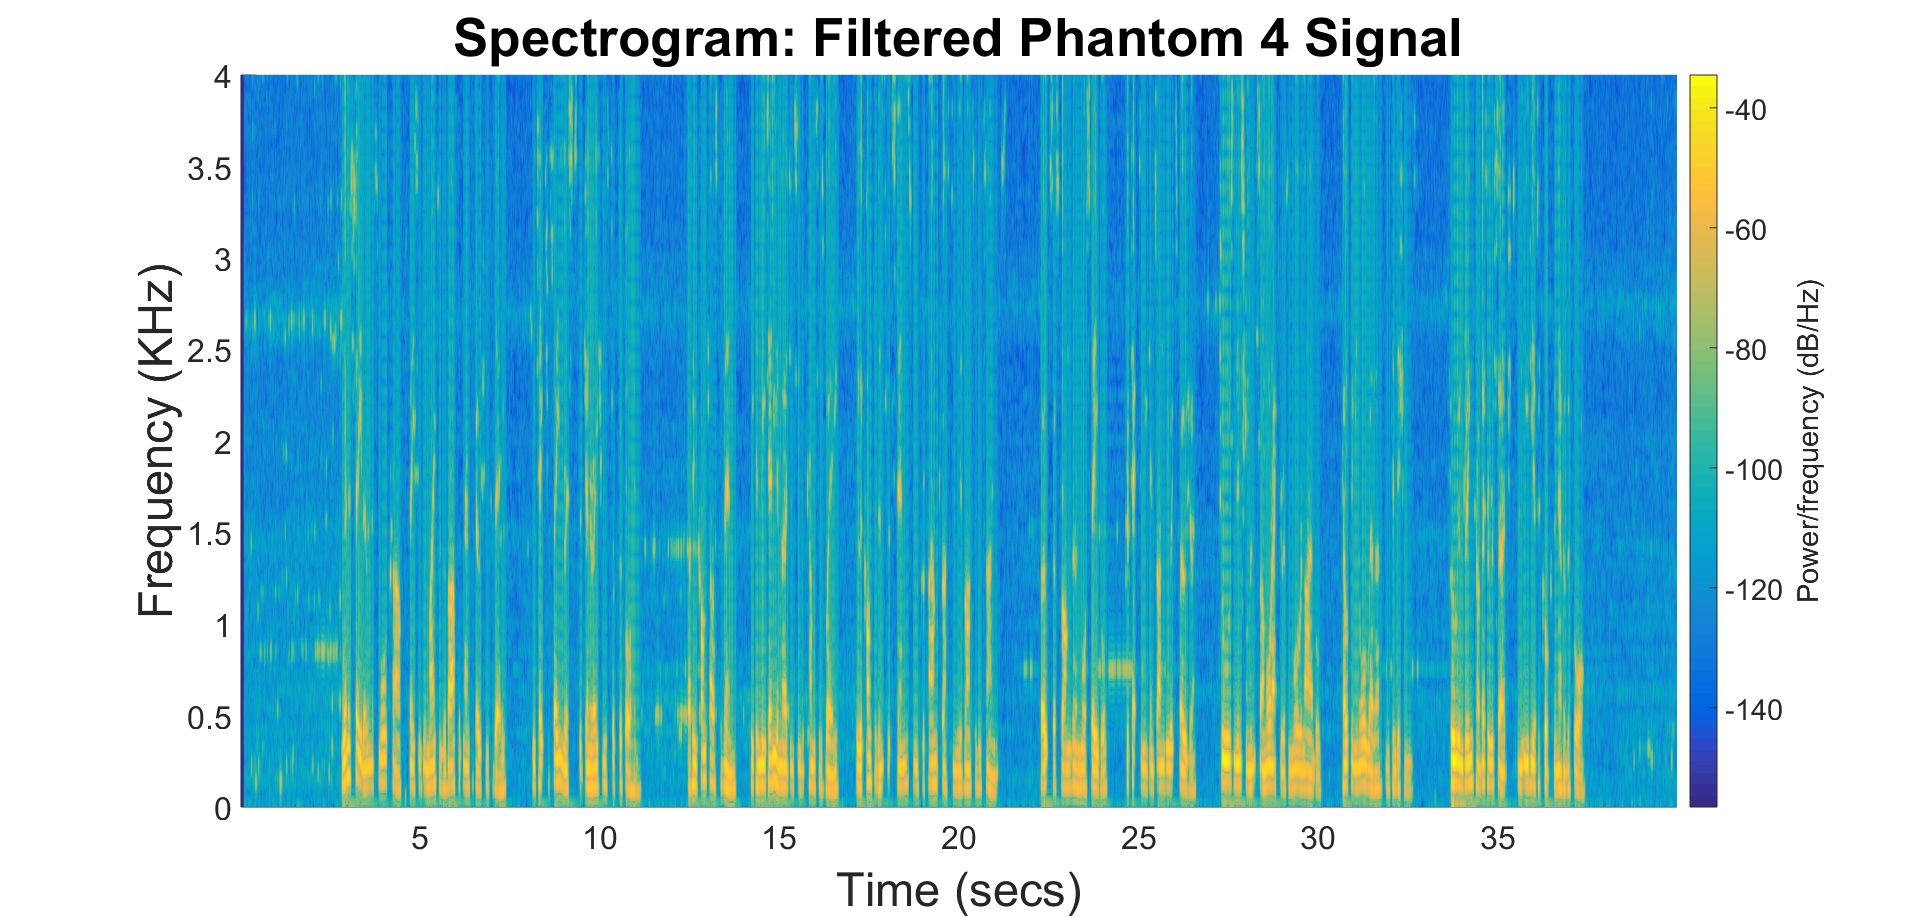
\includegraphics[width=\columnwidth]{final_ph4_filtered}
    \caption{Spectrogram of filtered signal}
    \label{fig:dirty}
\end{figure}

From figure \ref{fig:dirty}, it is clear that a substantial amount of the noisy has been removed by the implemented algorithm. Observed closely, it is possible to see tiny musical noise artifacts. 

To obtain a clearer description of the nature of the noise in phantom4.wav, we look at the spectrogram of just the noise, as illustrated in figure \ref{fig:noise}.

\begin{figure}[H]
    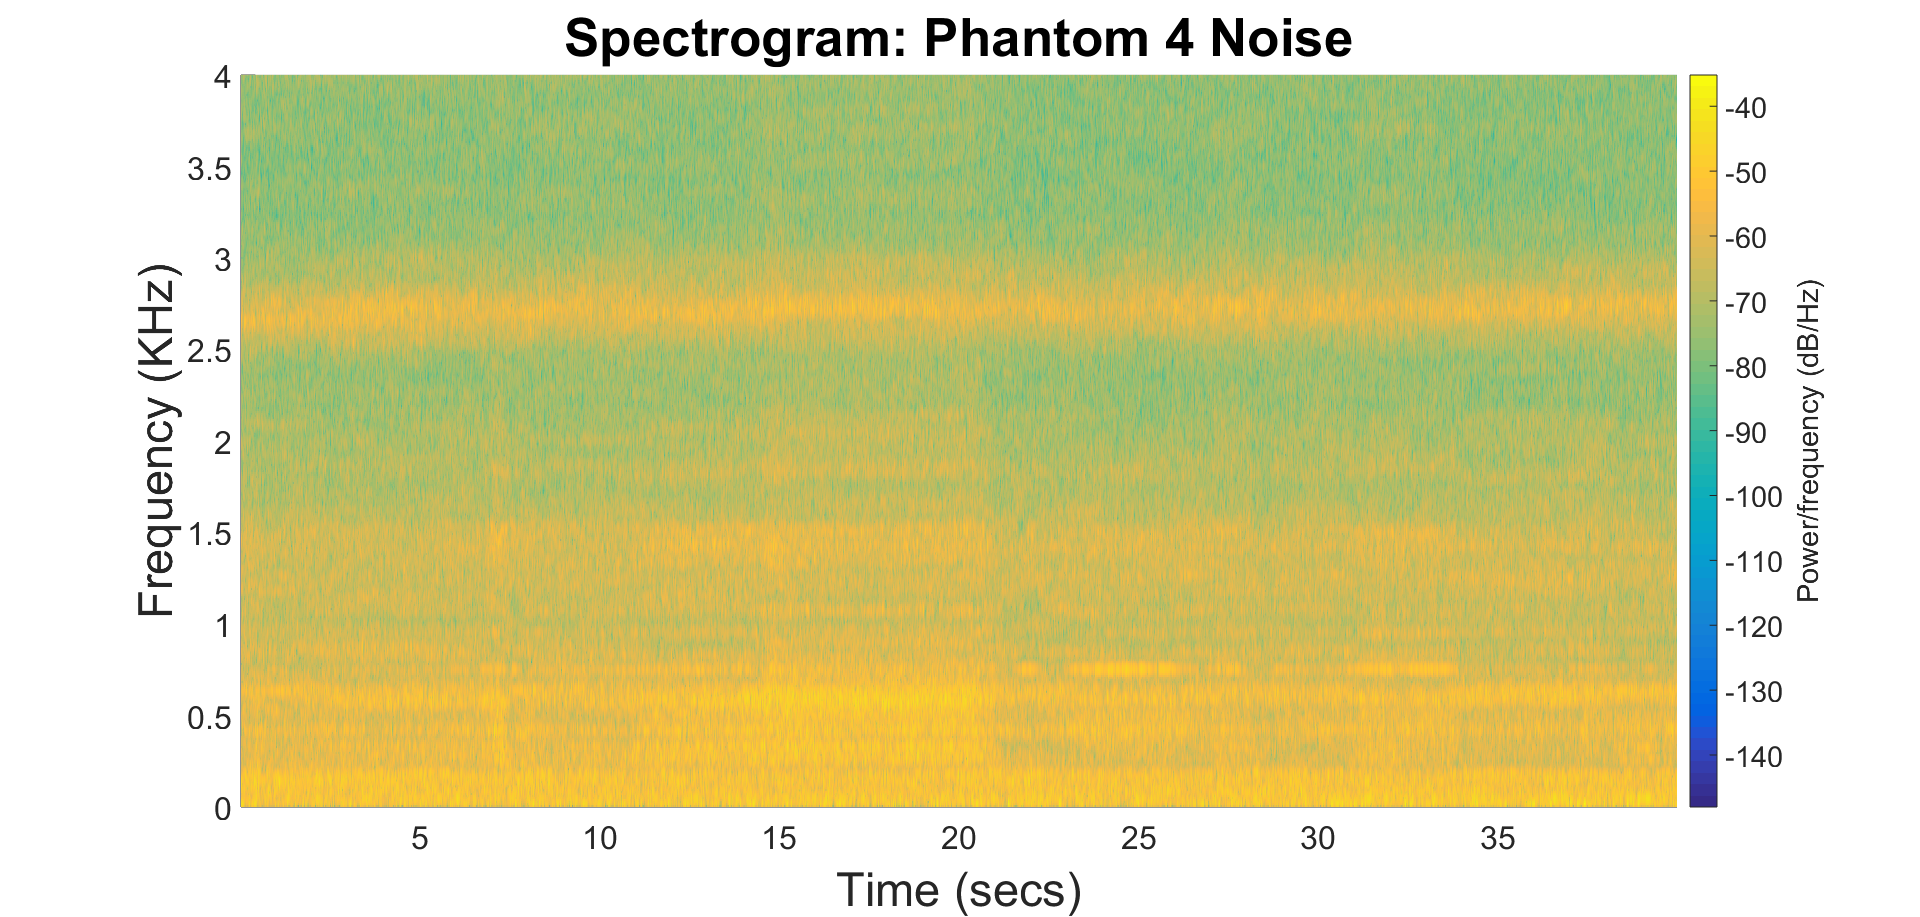
\includegraphics[width=\columnwidth]{final_ph4_noise}
    \caption{Spectrogram of noise in phantom4.wav}
    \label{fig:noise}
\end{figure}

From the Figure above it is clear that various types of noise exists within the corrupted signal:
\begin{enumerate}
    \item Background noise across all frequencies
    \item Stationary noise at specific frequencies: 2700Hz, 1500Hz and 130Hz
    \item Non-stationary noise between 500 and 750 Hz.
\end{enumerate}

The nature of the noise observed confirms that the techniques adopted in the final algorithm are justified. Background and stationary noise can be eliminated using the basic spectral subtraction algorithm. This however introduces musical noise that can be eliminated using the enhancements described above. The non-stationary noise is dealt with by the reduction in window length.

\subsection{Conclusion}

In conclusion, the basic spectral subtraction technique removes a significant amount of noise but fails to produce a high quality output when the SNR of the corrupted signal is low. To improve the performance, several enhancements have been proposed to increase the SNR although the best sounding algorithm does not combine all the enhancements. This is due to the subjective nature of the problem and because combining two enhancements that do not go well together causes the output to sound extremely distorted. 

\end{document}
